\documentclass[bachelor,german]{hgbthesis}
% Zulässige Class Options: 
%   Typ der Arbeit: diplom, master (default), bachelor, praktikum 
%   Hauptsprache: german (default), english
%%------------------------------------------------------------

%%% PACKAGES
\usepackage[utf8]{inputenc}

\usepackage[acronym, toc]{glossaries} % Acronym and Glossary

\usepackage{listings} % für inline code definitionen
\definecolor{codestringstylecolor}{rgb}{0.8,0.4,0}
\newcommand\codestringstyle{\color{codestringstylecolor}\ttfamily}
\newcommand\codekeywordstyle{\color{blue}\bfseries}
\lstdefinelanguage{JavaScript}{ % JavaScript definition für listings package
    keywords={typeof, new, true, false, catch, function, return, null, catch, switch, var, if, in, while, do, else, case, break},
    keywordstyle=\codekeywordstyle,
    ndkeywords={class, export, boolean, throw, implements, import, this},
    ndkeywordstyle=\color{darkgray}\bfseries,
    identifierstyle=\color{black},
    sensitive=false,
    comment=[l]{//},
    morecomment=[s]{/*}{*/},
    commentstyle=\color{purple}\ttfamily,
    stringstyle=\codestringstyle,
    morestring=[b]',
    morestring=[b]"
}
\lstdefinelanguage{json}{ % JSON definition für listings package
  stringstyle=\codestringstyle,
  morestring=[b]',
  morestring=[b]"
}

\lstdefinelanguage{yml}{ % YML definition für listings package
  keywords={true,false,null,y,n},
  keywordstyle=\codekeywordstyle,
  %basicstyle=\color{black}\bfseries, this makes the font bigger.
  sensitive=false,
  comment=[l]{\#},
  morecomment=[s]{/*}{*/},
  commentstyle=\color{purple}\ttfamily,
  stringstyle=\codestringstyle,
  moredelim=[l][\color{orange}]{\&},
  moredelim=[l][\color{magenta}]{*},
  moredelim=**[il][\color{red}\mdseries{:}\color{blue}\mdseries]{:},
  morestring=[b]',
  morestring=[b]",
  literate =    {---}{{\llap{\color{cyan}\mdseries-{-}-}}}3
                {>}{{\textcolor{red}\textgreater}}1     
                {|}{{\textcolor{red}\textbar}}1 
                {\ -\ }{{\mdseries\ -\ }}3,
}

\usepackage{amsmath} % Formeldarstellung

\usepackage{booktabs} % Tabellen
\usepackage{multirow} % Tabellen
\usepackage[table,xcdraw]{xcolor} % Tabellen
 % packages importieren

\graphicspath{{images/}}    % wo liegen die Bilder? 
\bibliography{literatur}  	% Angabe der BibTeX-Datei, % utf8-change
\makenoidxglossaries

\newglossaryentry{maths}
{
    name=mathematics,
    description={Mathematics is what mathematicians do}
}

\newacronym{lcm}{LCM}{Least Common Multiple}
\newacronym{IoT}{IoT}{Internet of Things}
\newacronym{DAPP}{DAPP}{Decentralized Application}
\newacronym{EVM}{EVM}{Ethereum Virtual Machine}


\newcolumntype{L}[1]{>{\raggedright\arraybackslash}p{#1}} % linksbündig mit Breitenangabe
\newcolumntype{C}[1]{>{\centering\arraybackslash}p{#1}} % zentriert mit Breitenangabe
\newcolumntype{R}[1]{>{\raggedleft\arraybackslash}p{#1}} % rechtsbündig mit Breitenangabe

%%%----------------------------------------------------------
\begin{document}
%%%----------------------------------------------------------

% Einträge für ALLE Arbeiten:
\title{lokkit - Einsatz von Blockchain und IoT}
\author{D.\ Hirzel und A.\ Schmid}
\studiengang{Informatik}
\studienort{Rotkreuz}
%\schulname{Lucerne University of Applied Sciences and Arts}
\schulname{Hochschule Luzern}
\abgabedatum{2017}{06}{09}
%\strictlicense  % erzeugt restriktive Lizenzformel

%%%----------------------------------------------------------
\frontmatter

\maketitle




\tableofcontents
%%%----------------------------------------------------------		

% \include{chapters/02_Selbststaendigkeitserklaerung} wird durch \maketitle bereits gemacht.
\chapter{Abstract d}
\label{cha:abstract_d}

Blockchain. Kryptowährungen. Dezentralisierte Datenbank. Internet of Things. Was sich für Laien anhört wie ein Auszug aus dem Computerduden, lässt die Herzen von so manchem Informatikstudenten höher schlagen. Bei diesen Begriffen handelt es sich nicht nur um Ausdrücke zur Geltendmachung der mentalen Überlegenheit durch Kenntnis von Fachbegriffen. Betont werden vor allem die rasant wachsende Anzahl vernetzter Geräte, die zunehmende Verteilung von Computersystemen \footnote{Referenz zu verteilten Energiesystemen, selbst fahrenden Autos o.Ä.?}, die immer grösser werdende Frage der Sicherheit derselben\footnote{Stichwort Globalisierung, Vernetzung} und die zunehmende Unlust von Unternehmen einander in der heutigen globalisierten Welt zu vertrauen\footnote{Kryptowährung \& BC}.

Pioniert wurde die Blockchain Technologie durch eine unter dem Pseudonym bekannte Person Satoshi Nakamoto. Dieser legte den Grundstein für diese sogenannten verteilten Ledger und implementierte im Jahr 2008 die heute immer noch bekannteste Blockchain mit gleich heissender Kryptowährung: Bitcoin. Neue Blockchain Implementationen unterstützen neben Kryptowährungen auch sogenannte \emph{Smart Contracts}. Diese erlauben es Benutzern Programmcode zu implementieren, der in der Blockchain abgelegt wird. Dieser Code kann beliebige Daten in diese verteilte Datenbank schreiben und wieder abfragen\footnote{Natürlich muss das bezahlt werden}. Dadurch, dass dieser Code, und auch die Daten, verteilt und somit von jedermann einsehbar sind, können Verträge unmissverständlich und öffentlich verfügbar in einem von Maschinen lesbaren Format definiert werden. Dies fördert die Transparenz und bedingt, dass beide Parteien zu ihrem besten Können auf die Erfüllung des Vertrags hin arbeiten.

Anwendungen, die diese Smart Contracts verwenden, nennt man \emph{\acrfull{DAPP}}. Diesebeschränken sich heute meist auf einfache Spiele\footnote{https://www.kingoftheether.com/thrones/kingoftheether/index.html}.


\cite{BlockchainRevolution}

Auch das Thema \acrshort{IoT} ist seit mehreren Jahren in aller Munde und wächst in den kommenden Jahren stark an. Gartner schätzt einen Zuwachs von 20.4 Milliarden Geräten bis 2020. Dies bringt neue Anforderungen an die Sicherheit mit - ein Aspekt, der eventuell durch die Blockchain-Technologie erfüllt werden kann.\cite{gartner.com_iot,BlockchainRevolution}

Im Rahmen dieser Bachelorarbeit wurden basierend auf ausgiebiger Recherche erwähnte Smart Contracts entwickelt und durch 


\chapter{Abstract e}
\label{cha:abstract_e}

Abstract goes here

%\printglossary[title=Abkürzungen und Definitionen, toctitle=List of terms]

\printnoidxglossary[type=\acronymtype]
 
\printnoidxglossary

%%%----------------------------------------------------------
\mainmatter         % Hauptteil (ab hier arab. Seitenzahlen)
%%%----------------------------------------------------------

%\chapter{Aufgabenstellung}
\label{cha:Aufgabenstellung}

Im diesem Kapitel wird die Aufgabenstellung aufgezeigt, die im Rahmen dieser 
Arbeit ebefalls erstellt wurde. Einzig die Schlagworte \emph{Blockchain},
\emph{\acrfull{IoT}} und den Bau eines Demonstrators waren vorgegeben.

Die \emph{Blockchain}-Technologie ist zurzeit stark im Trend. Sie benutzt verteilte
und dezentrale Rechennetzwerke und bietet dadurch bessere Sicherheit und geringere 
Kosten im Vergleich zu traditionellen Methoden.

Neue Blockchains unterstützen neben Crypto-Währungen auch sogenannte \emph{Smart Contracts},
die es dem Benutzer erlauben, Programme für die Blockchain zu implementieren. Diese
Art von Programm nennt man auch \emph{\acrfull{DAPP}}.

Auch das Thema \acr{IoT} ist in aller Munde und wächst in den kommenden Jahren stark an. Gartner 
schätzt Zuwachs von 20.4 Milliarden neuen Geräten bis 2020\footnote{http://www.gartner.com/newsroom/id/3598917}. Dies bringt neue Anforderungen an
die Sicherheit mit - ein Aspekt, der eventuell durch die Blockchain-Technologie erfüllt
werden kann.

Im Rahmen dieser Bachelorarbeit soll ein System entwickelt werden, das den IoT und Blockchain Aspekt
umsetzt und demonstriert.

\begin{itemize}
    \item \textbf{ Wieso sind Blockchain und IoT wichtig? Gartner Hype Cycler}
    \item \textbf{ Wieso schlaegt die Schule dieses Thema vor? }
    \item \textbf{ Was soll mit dem Demonstrator erreicht werden? }
\end{itemize}

\section{Anforderungen an den Demonstrator}
\label{sec:Anforderungen an den Demonstrator}
\begin{itemize}
    \item Der Demonstrator soll auf dem Schulareal ausgestellt werden können. 
    \item Der Demonstrator soll keine Abhängigkeiten nach Aussen haben (kein Internet benötigen)
    \item Der Demonstrator soll wiederverwendbar sein.
    \item Der Aufbau des Demonstrators sowie die Inbetriebnahme muss dokumentiert sein.
\end{itemize}

\section{Konkrete Aufgabenstellung}
\label{sec:Konkrete Aufgabenstellung}
Es soll ein System entwickelt werden, um Schließfächer an Personen zu vermieten. Jedes Schließfach muss elektronisch ver- und entriegelt werden können.

Der Benutzer soll über eine Oberfläche ein freies Schließfach reservieren können. Sobald der Benutzer der aktuelle Mieter eines Faches ist, kann er das Schloss per Knopfdruck öffnen und schliessen.

Im Fokus steht die Umsetzung mit einer geeigneten Blockchain.

\section{Ziele}
\label{sec:Ziele}
\begin{itemize}
    \item \textbf{ Was sind die Ziele die durch diese Arbeit erreicht werden sollen? }
    \item \textbf{ Was ist das Ziel des Demonstrators? }
\end{itemize}

\begin{itemize}
    \item Demonstrieren der Vorteile der Blockchain
    \item \dots
\end{itemize}


\section{Erwartete Resultate}
\label{sec:Erwartete_Resultate}

Ein lauffähiger Prototyp des Schliessfachvermietsystems.
%\chapter{Lösungsentwicklung}
\label{cha:Loesungsentwicklung}

\section{Recherche}
\label{sec:Blockchain}
\begin{itemize}
    \item \textbf{Informationssuche zu Beginn}
    \item \textbf{Was mit Blockchain alles gemacht werden kann}
    \item \textbf{Was wir mit Blockchain machen möchten}
    \item \textbf{technische Entscheidungen beschreiben}
    \item \textbf{Machbarkeitsanalyse lokkit}
    \item \textbf{Konzept verweist hierher für generelle infos und limitationen und Gründe für Entscheidungen}
\end{itemize}

referenz, verweise

\subsection{Verwendete Blockchain Implementation}
Dieses Projekt verwendet die open-source Blockchain-Implementation Ethereum\footnote{https://www.ethereum.org/} als Plattform für die Datenhaltung, die Business Logik in Form von Smart Contracts (vgl. \ref{subsec:Smart_Contracts} und \ref{subsec:lokkit_Smart_Contracts}) und einzige Interaktionsmöglichkeit für Benutzer mit dem System.

Ethereum ist die einzige Implementation einer Blockchain, die zum Start dieses Projektes eine funktionsfähige Plattform für eine Kryptowährung und Smart Contracts zur Verfügung stellt. Weitere Technologien, die in der Evaluationsphase analysiert wurden, sind Hyperledger, Bitcoin, Tendermint (nur ein consensus algo?), Nxt.

\subsubsection{Ethereum}
Die Finanzierung der Entwicklung der Ethereum Plattform durch ein Crowdfunding Projekt im Sommer 2014 ermöglicht. Der erste Release war ca. ein Jahr später am 30. Juli 2015. Die Implementation des lokkit Demonstrators wurde zu Beginn basierend auf der Version 1.5.9 von geth erstellt. Um neue Features wie Whisper v5 oder Mobile-Integration zu ermöglichen wurde die verwendete Version laufend an den aktuellen Entwicklungsstand der Ethereum Platform angepasst.
\paragraph{Konsensus}
Alle bisherigen Versionen des Ethereum Protokolls (Olympic, Frontier, Homestead) verwenden den \emph{Proof of Work} Algorithmus Ethash\footnote{https://github.com/ethereum/wiki/wiki/Ethash}, um Konsensus zu erreichen. Dies bedeutet, dass für jede Transaktion eine grosse Berechnung (proof) durchgeführt werden muss, bevor die Transaktion offiziell in die Blockchain eingetragen werden kann.

Für zukünftige Implementationen des Ethereum Protokolls war ein \emph{Proof of Stake} Algorithmus vorgesehen, um Konsensus zu erreichen, wurde jedoch kürzlich\footnote{} durch einen \emph{Proof of Authority} Algorithmus ersetzt. Grund dafür ist, dass die Kosten, eine Blockchain anzugreifen (bspw. um gewisse Blöcke neu zu schreiben durch erneute Berechnung der Hashes und zugehörigen Nonces), die einen Proof of Work Konsensus betreibt zusammen mit den Betriebskosten wachsen \footnote{https://www.coinmanual.com/proof\-stake/}\footnote{https://en.bitcoin.it/wiki/Proof\_of\_Stake}. Folglich kann ein Hochsicherheitssystem, wie es für Finanzdienste wie Banken oder Treuhänder benötigt würde, nur durch sehr hohe Betriebskosten realisiert werden. Ein wiederkehrendes Argument ist auch die Energie-Ineffizienz dieser Algorithmen. Aufgrund der benötigten hohen Rechenleistung sind Miner dazu geneigt ihre Rechenleistung zu konsolidieren und zu zentralisieren. Dies wird bei einem Anteil von 51\% Rechenleistung einer Entität zum Problem für den Konsensus. (\#TODO: see mail attachment "bda")

\paragraph{Solidity}
Solidity ist eine Programmiersprache, die auf der \acrfull{EVM} läuft, um Smart Contracts zu verfassen. Mehrere Sprachen konkurrieren mit Solidity, namentlich LLL und Serpent. Hierbei ist zu beachten, dass Solidity auf anderen Platformen wie Hyperledger Burrow durch eine Implementation der Ethereum VM ebenfalls lauffähig ist\footnote{https://github.com/hyperledger/burrow}.

\paragraph{Whisper}
\label{para:Whisper}
Whisper, auch analog zu der öffentlichen API \emph{shh} genannt, ist ein Kommunikationsprotokoll für \acrfull{DAPPs}. Nachrichten, die über das Whisper Protokoll verschickt werden, benutzen zur Übermittlung ebenfalls Ethereum Nodes, auf welchen das \emph{shh} Protokoll aktiviert wurde. Diese Nachrichten lösen keine Transaktionen auf der Blockchain aus. Wie auch die Transaktionen werden die Whisper Messages an alle Teilnehmer gesendet (broadcast), können aber mit einem \emph{topic} versehen werden, das es vereinfacht, erhaltene Nachrichten zu filtern. Jede Nachricht kann mit einer \acrfull{ttl} versehen werden, die angibt, wie lange die Nachricht verfügbar sein soll. Wenn diese Zeitspanne abläuft wird die Nachricht von den Ethereum Nodes nicht mehr weitergeleitet (Stale Message) und steht auf den Nodes, die die Nachricht bereits erhalten haben, nicht mehr zur Verfügung. So bietet das Whisper Protokoll eine einfache, leichtgewichtige Möglichkeit zur Echtzeit-Kommunikation für \acrshort{DAPPs}.

\#TODO: gehört das zu Konzeption? oder ganz streichen? Um das Whisper Protokoll auf einer Ethereum node zu aktivieren, muss geth mit dem \emph{-shh} Argument gestartet werden. Dies ermöglicht der jedoch Node erst, erhaltene Whisper Nachrichten von anderen Nodes weiterzuleiten. Damit die Whisper API über web3 zugänglich wird, ist zusätzlich der Eintrag \emph{shh}, in der mittels \emph{--rpcapi} angegebenen Liste der aktiven APIs, notwendig.
\begin{lstlisting}[language=bash,caption=Beispiel für die Aktivierung des shh Protokolls auf der Ethereum Node]
geth --shh
\end{lstlisting}
\begin{lstlisting}[language=bash,caption={Beispiel für die Aktivierung der web3, eth und shh API}]
geth --rpcapi "web3,eth,shh"
\end{lstlisting}
\begin{lstlisting}[language=bash,caption={Beispiel für die Aktivierung des shh Protokolls und der web3, eth und shh API}]
geth --rpcapi "web3,eth,shh"
\end{lstlisting}
\subparagraph{Whisper Identity}
\label{supara:Whisper_Identity}
\#TODO:obsolete. Um Whisper Nachrichten zu senden oder zu empfangen, kann eine Whisper Identity erstellt werden. Diese Identity wird während der Laufzeit des Programs gespeichert und beim beenden von bspw. \emph{geth attach} wieder gelöscht. Wird bei einer Nachricht ein Empfänger, in Form einer Whisper Identity, angegeben, wird die Nachricht verschlüsselt, sodass nur dieser die Nachricht entschlüsseln kann\footnote{http://web3js.readthedocs.io/en/1.0/web3-shh.html\#post}. Der Absender einer Nachricht, wie auch das Erstellen einer Whisper Identity an sich, ist optional. Das heisst, es können anonyme Nachrichten über Whisper verschickt werden, die keinerlei Rückschluss auf deren Ursprung machen lassen.

\subsubsection{Hyperledger}
Hyperledger ist ein Unterfangen mehrerer internationaler Firmen (\#TODOLinux Foundation, IBM, Intel etc), das zum Ziel hat, wichtige Funktionalität im Bereich von Blockchains zu erforschen und zu definieren, um schlussendlich einen industrieweiten offenen Standard für verteilte Ledgertechnologien zu erschaffen\footnote{https://wiki.hyperledger.org/community/welcomesheet}.

Zum Zeitpunkt des Starts dieses Projekts waren die Projekte 
\paragraph{Fabric}
\paragraph{Chaintool}
\paragraph{Burrow}

\subsection{Ethereum Testchain}
Die Ethereum Implementatoin stellt hart-kodiert zwei öffentliche Chain zur Verfügung. Zum einen die produktiv verwendete Chain \emph{Homestead}\footnote{}, auf der mit physischer Währung Ether gehandelt wird und die auch von mehreren Firmen produktiv verwendet wird\footnote{}. Zum anderen die Chain \emph{Ropsten}, die als aktuelle Testchain dient. Obwohl das Mining ebenfalls mit erheblicher Rechenleistung verbunden ist, kann Ether auf der Testchain nicht gegen \emph{echte} Währung eingetauscht werden. Grund daf¨r

\paragraph{Faucet Request}
\label{para:Faucet_Request}
Auf allen Testchains können sogenannte \emph{Faucet Requests}\footnote{https://blog.b9lab.com/when-we-first-built-our-faucet-we-deployed-it-on-the-morden-testnet-70bfbf4e317e}\footnote{https://ethereum.stackexchange.com/questions/84/what-public-test-networks-and-faucets-exist} gemacht werden, wodurch Ether erhalten werden kann. Dieser Ether wird von Entwicklern, die aktiv Mining betreiben, zur Verfügung gestellt (vgl. donate) und kann dann von weiteren Entwicklern verlangt werden. Meist ist ein Limit auf der Menge Ether pro Minute oder Adresse verhängt, das missbräuchliche Nutzung dieses Dienstes verhindern soll. Ziel dieser Faucets ist es, Entwicklern eine Möglichkeit zu geben, die öffentliche Testchain zu verwendet, ohne dabei selbst Mining betreiben zu müssen.

\subsection{Private Chain mit Ethereum}
Es ist möglich, unter Verwendung von Mobile Apps von Drittanbietern\footnote{Ethereum Status}, die \emph{Ropsten} Testchain anzusprechen. Durch Wunsch des Auftraggebers wurde eine Anbindung an die öffentliche \emph{Ropsten} Testchain ausgeschlossen, da die ständige Verfügbarkeit des Internets oder die Verfügbarkeit von Ether nicht gewährleistet sein kann. Folglich wurde eine private Blockchain auf der zur Verfügung gestellten Infrastruktur\footnote{Raspis} installiert. Um eine private Blockchain aufzusetzen wird ein Genesis Block benötigt und es müssen bestehende Nodes bekannt sein, die als peers hinzugefügt werden können.

\paragraph{Genesis Block}
In einer Blockchain wird der erste Block Genesis Block genannt. Hier werden initiale Kontostände (oft für die Entwickler oder Contributer) angelegt und unterschiedliche Konfigurationen bezüglich.
Um eine Verbindung zu einem Peer aufzubauen muss der Genesis Block auf beiden Nodes übereinstimmen. Wenn dies der Fall ist, kann der Synchronisierungsprozess beginnen.

\subsection{Konzept der Smart Contracts}
\label{subsec:Smart_Contracts}
''A computerized transaction protocol that executes the terms of a contract.``\cite{BlockchainRevolution}

Mit diesem Zitat kann grob das Ziel von Smart Contracts beschrieben werden. Verträge, die in einem maschinenlesbaren Format verfasst sind, können mit unmissverständlicher Präzision und ohne Interpretationsspielraum definiert werden. So ist es möglich, einen deterministischen, digitalen Vertrag zu verfassen.
Entgegengesetzt ist es nahezu unmöglich eine Menge von Smart Contracts angesichts einer unüblichen Situation deterministisch abzuarbeiten\footnote{http://www.ibtimes.co.uk/pwc-blockchain-expert-pinpoints-sources-ambiguity-smart-contracts-1575778}.

\subsubsection{Erstellung}
Um einen Smart Contract zu erstellen, wird dieser mittels einer geeigneten Programmiersprache formell definiert. Dieser geschriebene Programmcode kann durch eine Transaktion in die Blockchain eingesetzt werden, wobei Initialwerte für den Smart Contract angegeben werden. Man sprich hierbei vom erstellen einer Instanz des Smart Contracts, analog der Erstellung einer Instanz einer Klasse in der objektorientierten Programmierung. Bei der ausgelösten Transaktion gilt es zu beachten, dass dieser kein Empfänger angegeben wird; der Empfänger dieser Nachricht ist die Blockchain selbst. Wie bei jeder Transaktion eine gewisse Menge gas mitgegeben werden, damit die Operation abgeschlossen werden kann\footnote{echt? dachte das geht ohne explizit gas anzugeben}. Wenn der Code in die Blockchain eingesetzt wurde, erhält diese Instanz des Contracts eine Adresse, über die später mit dieser spezifischen Instanz interagiert werden kann.

Beim Erstellen eines Smart Contracts wird auch ein abi\footnote{Application Binary Interface} generiert. Dieses beschreibt die möglichen verfügbaren Attribute des Contracts und die Interaktionsmöglichkeiten (\#VGL. Funktionen) inklusive deren allfällige Parameter und Rückgabewerte (\#VGL. Interfacedeklaration in OO Sprachen).

\subsubsection{Lesezugriff}
Um ein Attribut auszulesen oder eine Funktion mit konstantem Rückgabewert auszuführen, kann diese über ein verfügbares Interface, wie die JavaScript console von geth, direkt aufgerufen werden. Bei Funktionen mit konstantem Rückgabewert ist zu beachten, dass diese nur auf der lokalen Node emuliert werden\footnote{} und es somit nicht möglich ist, eine Änderung in der Blockchain zu bewirken. Diese Funktionen haben folglich nur Lesezugriff. Allfällige Events, die in einer konstanten Funktion definiert wurden werden nicht ausgelöst.

\subsubsection{Schreibzugriff}
Wenn eine Funktion auf der Instanz aufgerufen wird, die eine Änderung in der Blockchain bewirkt, muss eine Transaktion ausgelöst werden. Der Sender der Transaktion muss dabei für die Kosten für gas und allfällige weitere Kosten (\#VGL. Bezahlbare Funktionen) aufkommen. Der Sender kann nicht nur ein Account sein, sondern auch ein weiterer Smart Contract, an dessen Adresse genügend Ether liegt, um die Transaktionskosten zu begleichen.

\paragraph{Bezahlbare Funktionen}
Einige Funktionen von Smart Contracts benötigen Ether, den man dem Aufruf hinzugibt. Dabei ist zu beachten, dass die gas Kosten und explizit gesendeter Ether nicht dasselbe sind. Wenn beispielsweise eine Dienstleistung oder Sache über einen Smart Contract verkauft werden soll, muss eine Menge Ether als Zahlungsmittel überweisen werden. Die Menge Ether ist im Smart Contract festgelegt und kann durch Inspektion des Programmcodes eingesehen werden. Sollte der Kunde zu wenig Ether schicken, kann der Smart Contract definieren, dass die Transaktion nicht erfolgreich ist und der Kunde sein Geld zurückerhält. Dazu kann die Transaktion selbst als nichtig erklärt werden und es muss nicht auf das Withdrawal Muster zuückgegriffen werden (vgl. Withdrawal Muster)

\subsubsection{Solidity}
Solidity ist eine Programmiersprache zur Erstellung von Smart Contracts auf der \acrfull{EVM}, die syntaktisch stark an JavaScript angelehnt ist. Sie kann auch auf anderen Blockchain Platoformen (wie Tendermint oder Counterparty für Bitcoin) verwendet werden. -> https://www.cryptocoinsnews.com/counterparty-brings-ethereum-smart-contracts-to-the-bitcoin-blockchain/\\Solidity wird, in Anlehnung auf den Ausdruck object-oriented, als contract-oriented bezeichnet, da die erstellenden Konstrukte in der Sprache \emph{contract} und nicht \emph{object} genannt werden. Inhaltlich beziehen sich die beiden Ausdrücke auf dasselbe Konzept.


\section{Konzeption}
\label{sec:Konzeption}
\begin{itemize}
    \item \textbf{Proof of concept zur Machbarkeitsanalyse aus vorherigem Kapitel}
    \item \textbf{Architektur, Aufbau inkl. Diagramme etc.}
    \item \textbf{Zu entiwckelnde Komponenten auflisten und Zuständigkeiten definieren. Bspw. Doorman ist eine Referenzimplementation, die es ermöglicht auf whispers zu hören. Alternativ kann anhand von folgender Beschreibung ein eigener doorman implementiert werden...}
    \item \textbf{Schnittstellen beschreiben. bspw. Whisper für webapp<->doorman Kommunikation erwähnen, aber \emph{nicht} deb eigenen Signaturmechanismus oder den Aufbau der ausgetauschten Nachrichten}
\end{itemize}

Die entwickelte DAPP ermöglicht es einem Owner ein Objekt über die Blockchain zu vermieten. Er kann dabei das Depot und die Mietkosten festlegen. Ein Renter kann dann dieses Objekt für eine bestimmte Zeit mieten. Die Abwicklung des Vertrages und dessen Kosten geschieht im Hintergrund in der Blockchain. Es gibt keinen Zwischenmann (z.B. Bank), der für die Überweisung zuständig ist, sondern das Geld fliesst direkt vom Renter zum Owner. 
Ein Objekt kann grundsätzlich alles sein: Ein elektrisches Fahrrad, eine Ferienwohnung oder einfach ein Schließfach. Es muss jedoch möglich sein ein Kontrollmechanismus anzubringen, der gleichzeitig ein Node in der Blockchain darstellt. Bei einem elektrischen Fahrrad wäre es z.B. möglich einen Minicomputer im Fahrgestellt zu montieren, welcher den Akku aktiviert oder deaktiviert und über eine Sim-Karte mit der Blockchain synchronisiert. Möchte ein Benutzer das Fahrrad verwenden, so müsste er dieses zuerst über die Blockchain mieten und erst dann kann er den Akku aktivieren. Die Mietkosten würden direkt dem Anbieter des Fahrrades überwiesen werden.

\begin{figure}
\centering
\includegraphics[width=.95\textwidth]{Mobile_Konzept}
\caption{Das Mobile-Konzept, dessen Umsetzung möglich ist}
\label{fig:Mobile_Konzept}
\end{figure}

\vspace{1em}
Als Proof of Concept wurde in dieser Arbeit einen Demonstrator entwickelt. Es handelt sich um ein Schliessfach-Vermietsystem, welches als Backend eine private Blockchain nutzt. Jedes Fach hat ein elektrisches Türschloss, welches über ein Raspberry PI durch die Blockchain kontrolliert wird. Ein Schließfach und ein Raspberry PI bilden zusammen eine Einheit (ein Node der privaten Blockchain). Das erste Schliessfach erstellt ausserdem ein WLAN Hotspot, auf den alle anderen Einheiten verbinden. Der Demonstrator verfügt über 3 Einheiten, welche sich zum Hotspot verbinden. Die Anzahl der Einheiten ist nicht beschränkt, solange sie in der Reichweite des WLAN Hotspots befinden. Alle Einheiten zusammen bilden die private Blockchain. 

\subsection{Interaktion mit dem Demonstrator}
\label{sec:Interaktion mit dem Demonstrator}

Ein Benutzer muss sich zuerst als einen weiteren Node mit der Blockchain verbinden. Anschliessend kann er über die entwickelte Webapp (DAPP) mit dem System interagieren. 

\vspace{1em}\noindent
Folgende Interaktionen sind möglich.

\vspace{1em}\noindent
\textbf{Als Owner}
\begin{itemize}
    \item Neues Rentable (Objekt) erfassen
    \item Bestehende Rentable deaktivieren/aktivieren/zerstören
\end{itemize}

\vspace{1em}\noindent
\textbf{Als Renter}
\begin{itemize}
    \item Nach Rentables suchen (Discover)
    \item Informationen und Verfügbarkeit eines Rentables prüfen
    \item Ein Rentable reservieren (rent)
\end{itemize}

\vspace{1em}\noindent
\textbf{Als aktueller Renter (current renter)}
\begin{itemize}
    \item Sperren und Entsperren des Rentables (Lock/Unlock)
    \item Zurückgeben des Schließfachs (Unclaim)
    \item Verlängern der aktuellen Reservation (Emergency)
\end{itemize}

\subsection{Regeln}
\begin{enumerate}
    \item Hat zum aktuellen Zeitpunkt niemand das Rentable reserviert, so ist der Owner gleich dem Renter.
    \item Es gibt keine Reservationsüberlappungen
    \item Eine aktive Reservation kann mittels \emph{Emergency} verlängert werden. Steht die Verlängerung im Konflikt mit einer nächsten Reservation, so wird der Startzeitpunkt der Reservation nach hinten verschoben. Wird im Fallbeispiel ... erläutert.
    \item ...
\end{enumerate}


\subsection{Fallbeispiele}
\label{sec:Fallbeispiele}
Die folgenden Fallbeispiele erläutern das Zusammenspiel der Interaktionen und die Verschiebung der priviligierten Rechte entlang der Zeitachse.

\subsubsection{Normal-Fall}
In Abb.~\ref{fig:Cases}\,(a) reserviert Benutzer A das Schliessfach von $t_{R1}$ bis $t_{R2}$ zum Zeitpunkt $t_0$. Das Deposit und die Mietkosten werden ihm somit abgezogen.
Zum Zeitpunt $t_{R1}$ wird Benutzer A zum \emph{Current Renter} und besitzt dadurch privilegierten Zugriff. Er kann jetzt das Schliessfach öffnen (Unlock) und schliessen (Lock). Nach einer gewissen Zeit noch vor Ablauf der Reservation, entschliesst sich Benutzer A das Schliessfach wieder abzugeben (Unclaim), da er es nicht mehr benötigt. Die Reservation wird somit auf diesen Zeitpunkt gekürzt und Benutzer A erhählt sein Deposit und die Mietkosten für die ungenutzte Zeit zurück. Die priviligierten Rechte werden umgehend wieder an den Owner abgegeben.

\begin{figure}
\centering\small
\setlength{\tabcolsep}{0mm}	% alle Spaltenränder auf 0mm
\begin{tabular}{c@{\hspace{12mm}}c} % mittlerer Abstand = 12mm
  \includegraphics[width=.45\textwidth]{Case-Normal} &
  \includegraphics[width=.45\textwidth]{Case-No-Unclaim} \\
  (a) & (b)
  \\[1em]	%vertical extra spacing (4 points)
  \multicolumn{2}{c}{\includegraphics[width=.45\textwidth]{Case-Emergency}}\\
  \multicolumn{2}{c}{(c)} 
\end{tabular}
%
\caption{Verschiedene Fälle -- 
Normal-Fall (a), Keine-Rückgabe (b),
Emergency-Fall (c).}
\label{fig:Cases}
\end{figure}

%\begin{figure}
%\centering
%\includegraphics[width=.95\textwidth]{Case-Normal}
%\caption{Normal-Fall}
%\label{fig:Case-Normal}
%\end{figure}

\subsubsection{Reservationsende ohne Betätigung der Rückgabe}
Wie im Normal-Fall beschrieben, ist Benutzer A momentaner Renter (current renter) des Schliessfaches. Anstelle jedoch das Schließfach wieder zurückzugeben, lässt er die Reservationszeit auslaufen. Zum Zeitpunkt $t_{R2}$ werden ihm die Rechte entzogen und er erhält keine Rückerstattung des Deposits. Es liegt also in Benutzer A seinem Interesse, alle eingeschlossenen Gegestände vor Ablauf der Reservation aus dem Schließfach zu nehmen und dieses zurückzugeben (Unclaim). Siehe Abb.~\ref{fig:Cases}\,(b) als Illustration.

\subsubsection{Emergency zum Verlängern der Reservationsdauer}
Der Benutzer A sollte immer einen Buffer in die Reservationszeit einplanen, damit er das Schließfach auch noch bei Zugsausfall oder einem Autounfall rechtzeitig vor Reservationsablauf erreichen kann. In äußersten Notfällen kann es trotzdem vorkommen, dass der Benutzer A nicht rechtzeitig seine Affären aus dem Schließfach nehmen kann und aus diesem Grund hat er die Möglichkeit eine \emph{Emergency} auszulösen. Die Emergency ist entsprechend kostenintensiv und sollte deswegen nur in Notfällen und abhängig vom Wert der Gegenstände im Schließfach in Erwägung gezogen werden. 
Die Emergency verhindert den Ablauf der aktuellen Reservation und überschreibt allenfalls nachfolgende Reservationen. Betroffene Reservationen erhalten einen Teil der Einnahmen durch die Emergency als Entschädigung. Die Abbildung \ref{fig:Cases}\,(c) veranschaulicht dieses Scenario.

\subsubsection{Fall von Schäden}
Benutzer A reserviert wie im Normal-fall ein Schliessfach. Zum Zeitpunkt t1 will er das Schliessfach öffen (Unlock), dieses reagiert jedoch nicht. Er muss nun Kontakt mit dem Owner aufnehmen und die Sache klären. Auf jeden Fall sollte er nun das Schliessfach zurückgeben (Unclaim) um die Kosten niedrig zu halten, im Falle, dass sich der Owner nicht auffinden lässt oder dieser kein Interesse zeigt.

Im Rahmen dieser Arbeit wurde auch ein Konzept überlegt, wie solche Probleme vermindert werden könnten. Durch Einführen eines Review Systems, wo Benutzer die Owner beurteilen können. Owner mit einer guten Bewertung (Score) wären dann vertrauenswürdiger.

\begin{itemize}
    \item \textbf{ Wie funktioniert unsre Loesung? }
    \item \textbf{ Was ermoeglicht unsere Loesung? }
    \item \textbf{ Wie sicher ist das System? }
    \item \textbf{ Was sind moegliche Angriffe? }
    \item \textbf{ Wie stehts mit der Verfuegbarkeit?}
    \item \textbf{ Gibt es Restrictions?}
    \item \textbf{ Was sind die Staerken und Schwaechen dieser Loesung? }
    \item \textbf{ Wie ist der Ablauf? Was geschieht wann?\ref{sec:Fallbeispiele}}
    \item \textbf{ Was kann der Benutzer machen? \ref{sec:Interaktion mit dem Demonstrator}}
    \item \textbf{ Wie sind die Regeln? Wer kann reservieren und wann? Was passiert, wenn die Reservation ablauft? Wer haftet? Was ist, wenn das Schliessfach beschaedigt ist und ich es nicht antreten kann?\ref{sec:Fallbeispiele}}
    \item \textbf{ Wie sieht das Kostenmodel aus? Beispiele und Scenarien?}
    \item \textbf{ Wer nutzt unsere Loesung? }
    \item \textbf{ Warum nutzt man unsere Loesung?}
    \item \textbf{ Was sind Scenarien, wo unsere Loesung zum einsatz kommen wuerde?}
    \item \textbf{ Wie ist der grobe Aufbau?}
    \item \textbf{ Was fuer Technologien setzen wir ein und weshalb Blockchain?}
    \item \textbf{ Wie ist die Interaktion mit dem Benutzer? Kontextdiagramm? Es gibt mehrere Benutzer und Rollen.}
    \item \textbf{ Was brauchts um diese Loesung um zu setzten? Smart Contracts, Blockchain, Hardware, WebUI }
    \item \textbf{ In welche Komponenten ist das System aufgeteilt. Was sind die eizelnen Funktionen?}
    \item \textbf{ Was sind die Abhaengikeiten unseres Systems?}
    \item \textbf{ Wie sehen die Schnittstellen aus?} 
    \item \textbf{ Was fuer Technologien werden eingesetzt?} 
    \item \textbf{ Wie sieht das Design der Komponenten aus? Erweiterbar? Wartbar?} 
    \item \textbf{ Wie sieht das User Interface aus?} 
    \item \textbf{ Welche Libraries verwenden wir? Was haben wir entwickelt?}
    \item \textbf{ Wie wird das System deployed?}
    \item \textbf{ Kann man updates fahren?}
    \item \textbf{ Schrittanleitung zur Installation?}
\end{itemize}
    

\section{Implementation (Komponenten)}
\label{sec:Implementation}
Nachfolgend werden getroffene Entscheidungen zum Entwurf und zur Implementation der Komponenten beschrieben. Angetroffene Probleme werden vorgestellt und und deren Lösung erklärt\footnote{Konkrete technische Hindernisse mit Verweise auf Anhang zu Open Source changes/contributions oder auch technische Limitation wie bspw. go-ethereum mobile hat keine whisper API}.

Allfällige Abweichungen zur Konzeption (vgl. \ref{sec:Konzeption}, bspw. teilweise oder fehlende Implementation, werden erwähnt und, wo angebracht, werden weitere Überlegungen und Möglichkeiten zur Erweiterung der Komponenten erläutert.

\subsection{Smart Contracts}
\label{subsec:Smart_Contracts}
Die Smart Contracts, die in Solidity implementiert wurden, werden nachfolgend erläutert. Diese Implementationen bilden das Rückgrat der Applikation. Sie bilden die Business Logik in Code Form ab und dienen als einzige Interaktionsmöglichkeit mir der Datenbank in der Blockchain.

(vgl. http://solidity.readthedocs.io/en/latest/introduction-to-smart-contracts.html)

\#WICHTIG!!
Erwähnen der shortcomings, da unsere Contracts eine nicht vordefinierte Anzahl Iterationen haben. Dies kann aufgrund des Block-Gas limits zu stalling führen. Auch lese-Operationen, die aus anderen Smart-Contracts aufgerufen werden können diesen zum stallen bringen. -> http://solidity.readthedocs.io/en/develop/security-considerations.html\#gas-limit-and-loops

\subsubsection{Generell}
\paragraph{Datenhaltung}
In einem Smart Contract können Daten in der Blockchain auf unterschiedliche Arten gespeichert werden: \emph{Storage}\footnote{http://solidity.readthedocs.io/en/latest/miscellaneous.html\#layout-of-state-variables-in-storage} oder \emph{Events} (auch \emph{Logs} genannt). Storage ist ein einfacher Schlüssel-Werte-Paar Speicher, worauf alle Instanzvariablen eines Smart Contracts gespeichert werden, die zwischen verschiedenen Funktionsaufrufen persistiert werden müssen (vgl. reservations Feld für Rentables). Ein Smart Contract kann nicht ausserhalb seines zugewiesenen Speicherbereichs operieren. Zugriffe auf diesen Speicher sind teuer. So soll verhindert werden, dass grosse Speichermengen in der Blockchain verwendet werden. \footnote{http://solidity.readthedocs.io/en/latest/introduction-to-smart-contracts.html?highlight=memory\#storage-memory-and-the-stack}. Ausgelöste Events werden in der Blockchain in Form von Transactionlogs gespeichert. Diese Logs sind sehr günstig (vgl. gas price) anzulegen, können aber von einem Smart Contract nicht gelesen werden \footnote{http://jonathanpatrick.me/blog/ethereum-compressed-text}. Über die web3 API kann auf die so erstellten Logs zugegriffen werden \#TODO: insert Beispiel.

Somit kann gesagt werden, dass wenn eine Instanz eines Smart Contracts persistent Daten speichern und diese Daten in einem späteren Funktionsaufruf abfragen möchte, zwingend Storage Speicher verwendet werden muss. Damit die Konsistenz der Reservationen eines mietbaren Objektes gewährleistet werden kann, muss der Rentable Smart Contract die Möglichkeit besitzen, bestehende Reservationen abzufragen. Daher ist es unumgänglich für den Rentable Smart Contracts Storage Speicher für die Datenhaltung der Reservationen zu verwenden. Auch für den Rentable Discovery Smart Contract ist es zwingen notwendig, dass die registrierten Rentable Instanzen abgefragt werden können. Somit ist auch bei diesem Storage Speicher für die Datenhaltung der Adressen zu verwenden.

\subsubsection{Rentable}
\label{subsubsec:Rentable}
Vgl. \ref{sys_subsubsec:Rentable}
\\Damit alle mietbaren Objekte logisch unabhängig von einander sind, wurde der primäre Smart Contract so entworfen, dass für jedes mietbare Objekt eine separate Instanz dessen erstellt werden muss (vgl. contract Instanz erstellen). Die in der Blockchain liegende Funktionalität beinhaltet nur das Mieten, und die damit verbundene Monetären Transaktionen. Der Smart Contract weist dabei keine lokkit-spezifische Funktionalität auf. Bei dem Design wurde darauf geachtet, die Funktionalität zu abstrahieren, um es Autoren zu ermöglichen, weitere Dienste zu erstellen, die auf dem Konzept der mietbaren Objekte basiert. Diese darauf aufbauenden Dienste können auch ausserhalb des lokkit Systems bestehen und können gänzlich inkompatibel zu diesem sein.

\paragraph{Withdrawal Muster}
Bei Transaktionen, die einen Account zum Ziel haben, werden die gas-Kosten automatisch vom Sender beigefügt (\#TODO: quelle+beispiel+formel). Ist das Ziel aber eine Funktion eines Smart Contracts (wie es bei Rentable.rent der Fall ist) oder ein Smart Contract selbst\footnote{Default Function: https://ethereum.stackexchange.com/questions/15420/how-to-send-ether-to-contracts-address/15450\#15450}, so kann der Smart Contract, der die Transaktion erhält, Code ausführen, der vom initialen Sender der Transaktion bezahlt werden muss (vgl. gas). Um dies zu verhindern, sollte nicht Ether an eine Adresse überwiesen werden, von der nicht bekannt ist, ob sie ein Smart Contract oder ein Account ist\footnote{https://github.com/ethereum/go-ethereum/wiki/Contracts-and-Transactions}.

\subparagraph{Beispiel}
Sei A eine Instanz eines Rentable Contracts, der das Withdrawal Muster implementiert. Wenn ein Depot zurückerstattet wird, überweist A Ether nicht direkt an eine Zieladresse, B. Stattdessen merkt sich A die Menge Ether, die B zusteht und stellt die Möglichkeit zur Verfügung, dass B Ether vom Smart Contract abheben kann. Dies findet mittels einer Transaction auf \emph{withdraw} statt, die von B ausgelöst werden muss. Die gas-Kosten für die primär von B ausgeführte \emph{withdraw} Funktion sind vernachlässigbar und werden durch die zurückerhaltene Menge Ether kompensiert. Der Vorteil, wenn die Transaktion von B gestartet werden muss, ist, dass B für die etwaigen zusätzlichen gas-Kosten aufkommen muss, sollte B ebenfalls ein Smart Contract sein. 

\#möglicherweise ein bildli zeichnen oder beispielcode einfügen

\paragraph{Re-Entrancy}
Hierbei handelt es sich um ein Muster, das angewendet wird, wenn in einem Smart Contract ein interner Zustand existiert, der die Menge an Ether speichert, der \emph{anderen} zusteht und eine Möglichkeit besteht, diese Menge Ether zu entnehmen (\#VGL. Withdrawal Muster). Beispiele für zurückzuerstattenden Ether kann bspw. Depots wie bei lokkit oder ein Gebot in einer Auktion\footnote{http://solidity.readthedocs.io/en/develop/security-considerations.html\#re-entrancy} sein.

\subparagraph{Beispiel}
Sei A eine Instanz eines Rentable Contracts, der diesen erwähnten internen Zustand speichert und somit das Withdrawal Muster implementiert. Unter der Annahme, dass die Zieladresse für die Rückerstattung ein beliebiger Smart Contract B ist, kann B A angreifen. Wenn eine Transaktion ausgelöst wird, wird jeweils nicht nur der Betrag in Ether überwiesen, sondern, sollte das Ziel ein Smart Contract sein, auch Code ausgeführt. Das heisst, dass B auf eine eingehende Überweisungen reagieren kann\footnote{solidity default function: function () payable\{\}} und ihrerseits erneut die Transaktionsfunktion von A aktivieren kann (\#VGL. Withdrawal Muster), bevor die Kontrolle an den ursprünglichen Aufruf von A zurückgegeben wird\footnote{daher re-entrancy, da die Funktion mehrere Male ausgeführt wird}. Wenn der Zustand von A noch nicht geändert wurde, wird der Betrag erneut gesendet, bis A keinen Ether mehr zur Verfügung hat.

\subparagraph{Implementationsbeispiel}
Um mehrfaches Überweisen von Ether zu verhindern, ist es unvermeidbar, zuerst den internen Status des Vertrags zu ändern, bevor Ether überwiesen wird. Die \emph{total} zur Verfügung stehende Menge Ether eines Smart Contracts wird in der Blockchain gehalten und ist Teil des Konsensus. Es ist somit nicht möglich, dass mehr Ether ausgegeben wird als in dem jeweiligen digitalen Vertrag vorhanden ist. 

Im Codebeispiel \ref{lst:withdraw_erroneous} kann die \emph{send} Anweisung in Zeile zwei mehrmals ausgeführt werden, da das deposit erst zurückgesetzt wird, sobald die Übertragung erfolgreich war. Dabei ist zu bemerken, dass die Funktion .send(...) die Kontrolle an die default-Funktion\footnote{vgl. default-funktion} des Zielvertrags übergibt und deren Code ausgeführt wird.
\begin{lstlisting}[language=javascript,caption={fehlerhaftes Code Snippet},label={lst:withdraw_erroneous}]
    function withdraw() {
        if (msg.sender.send(deposit[msg.sender])) {
            deposit[msg.sender] = 0;
        }
    }
\end{lstlisting}

Im Codebeispiel \ref{lst:withdraw_good} wehrt die dritte Zeile die Re-Entrancy Attacke ab, da der interne Kontostand zurückgesetzt wird, bevor die Transaktion ausgelöst wird. Auch hier wird der default-Funktion\footnote{vgl. default-funktion} des Zielvertrags die Kontrolle übergeben. Im Fall, dass diese aber erneut die \emph{withdraw} Funktion aufruft, wird diese keine erneute Transaktion auslösen (msg.sender.transfer(0) wird keine Transaktion auslösen\footnote{}).
\begin{lstlisting}[language=javascript,caption={empfohlenes Code Snippet},label={lst:withdraw_good}]
    function withdraw() {
        var currentRefund = deposit[msg.sender];
        deposit[msg.sender] = 0;
        msg.sender.transfer(currentRefund);
    }
\end{lstlisting}

\paragraph{Weitergehende Überlegungen}
Mögliche Verbesserungen bzgl. der momentanen Implementation.

\subparagraph{Migrations}
Um neue oder geänderte Funktionalität in Smart Contracts zur Verfügung zu stellen, muss die Datenhaltung von der Businesslogik entkoppelt werden. Grund dafür ist, dass wenn ein neuer Smart Contract als Interaktionsmöglichkeit in der Bockchain steht, Daten, die durch Transaktionen in der Blockchain entstanden sind, nicht einfach übernommen werden können, wie beispielsweise Reservationen. Diese Daten könnten prinzipiell durch den Besitzer des Objekts migriert werden. Das würde aber bedeuten, dass in der Blockchain der Besitzer des Objekts im Namen seiner Mieter Reservationen tätigt, was seinerseits wiederum eine Sicherheitslücke und mögliches Missbrauchspotential seitens des Besitzers bedeutet.

Truffle Migrations?


\subsubsection{RentableDiscovery}
Für jede Interaktion mit einem mietbaren Objekt muss dessen Adresse bekannt sein. Das heisst, um administrative Aufgaben am Objekt wahrzunehmen, diese zu mieten oder mit ihnen über das Whisper Protokoll zu interagieren. Diese benötigte Adresse kann manuell gefunden und eingegeben werden, beispielsweise durch eine Aufschrift auf dem Objekt oder durch einen QR Code\footnote{vgl webapp}. Alternativ zu diesem Ablauf wurde eine Utility entworfen, die das Erstellen und Finden von mietbaren Objekten erleichtert.
\\Der RentableDiscovery Contract stellt eine Möglichkeit zur Verfügung, Rentable Contracts in der Blockchain einzutragen, ohne direkt mit dem Rentable Contract zu interagieren, ähnlich dem Factory Pattern aus der objektorientierten Programmierung\footnote{http://www.oodesign.com/factory-pattern.html}. Diese Factory hat den Vorteil, dass damit erstellte Rentables direkt der Discovery bekannt sind und gefunden werden können. Es existiert auch die Möglichkeit, bestehende Rentables nach deren manuellen Erstellung nachzutragen. Die zu bezahlenden Kosten in gas sind beim neuen Erstellen niedriger als beim nachträglichen Hinzufügen, da nicht zuerst die Existenz der Adresse geprüft werden muss.

\#TODO: einfügen einer Formel für gas-Kosten wäre nicht schlecht.

\paragraph{Weitergehende Überlegungen}
Durch Verwendung eines QR Code Scanners im Webapp wird diese Funktionalität obsolet gemacht. Sie wird in lokkit nicht mehr auf der Oberfläche eingesetzt. Sie kann optional verwendet werden, um eine Übersicht über bestehende Rentables zu haben, und dabei nur eine einzelne Adresse (die der RentableDiscovery) zu speichern.

In Zukunft könnten bei Bedarf Rentables mittels dieser RentableDiscovery in logische Gruppen unterteilen werden, um die Darstellung zu erleichtern. Weiter könnte ein dynamisches Angebot von Rentables zur Verfügung gestellt, indem Abfragen nicht über manuelle QR Codes sondern über eine (oder mehrere) RentableDiscovery gestellt werden.

\subsection{Real-Time Kommunikationsschnittstelle}
Für Implementationsdetails, vgl. \ref{subsec:Real_Time_Kommunikationsschnittstelle}

Da die Block Time in der Ethereum Blockchain etwa 12 Sekunden beträgt\footnote{https://blog.ethereum.org/2014/07/11/toward-a-12-second-block-time/}, sind Transaktionen nicht nützlich, um in Echtzeit mit einem gemieteten Objekt zu interagieren. Auch die dabei anfallenden Kosten einer Transaktion\footnote{Diese Kosten sind gering für einfaches Signaling mit Smart Contracts.} sind zu begleichen und speziell bei wiederholtem Senden der Signale nicht zu verachten. Auch dient die Persistenz in der Blockchain all dieser Interaktionen keinem Nutzen, da aus dem Smart Contract bekannt ist, dass der Benutzer Zugriff auf das Gerät hat.

Daher wurde, um mit mietbaren Objekten (vgl. \ref{subsec:lokkit_Smart_Contracts}) während des gemieteten Zeitraums in Echtzeit zu interagieren, das Protokoll Whisper v5\footnote{vgl. \ref{para:Whisper}}\footnote{Auch Whisper v2 wurde angeschaut, aufgrund der nicht vorhandenen Unterstützung in der go-ethereum mobile API fallen gelassen und für die status-go mobile API mit Whisper v5 Unterstützung ausgetauscht. VGL. Anhang} verwendet. Whisper v5 erlaubt die Übermittlung von textbasierten Nachrichten mit eingebautem Sicherheitsmechanismus zur Verschlüsselung und optionale Signatur von Nachrichten. Diese Nachrichten müssen entweder symmetrisch oder asymmetrisch verschlüsselt werden\footnote{https://github.com/ethereum/go-ethereum/wiki/Whisper-Usage}.

Da Whisper v5 die einzige Möglichkeit zur Echtzeitkommunikation in der Ethereum Blockchain ist, gibt es keine Alternativen dazu.

\subsubsection{Verteilung}
\ref{subsubsec:Verteilung}
Das Whisper v5 Protokoll setzt für jede Nachricht einen Schlüssel (symmetrisch oder asymmetrisch) und ein Topic (4 bytes) voraus. Whisper Abos müssen mindestens ebenfalls einen Schlüssel und ein Topic als Filter beinhalten. Um neuen Teilnehmern zu er möglichen auf diese Nachrichten zu hören und solche zusenden, wird ein symmetrischer Schlüssel mit dem Passwort \emph{lokkit} erstellt. Dieser Schlüssel muss nicht geheim gehalten werden, da der Inhalt der Nachricht nicht sicherheitsrelevant ist\footnote{Sollte in Zukunft die Anforderung an verschlüsselte Commands gestellt werden, vgl Anhang \#TODO: generate asymmetric key + in smart contract schreiben. --> vgl. Sicherheitsaspekte. Müsste transaction auslösen von doorman}. Als Topic werden die ersten 4 Bytes der sha3 Checksumme der Adresse des Mietbaren Objektes mitgeschickt. Basierend auf diesen beiden Eigenschaften kann der Doorman (vgl. \ref{subsec:Doorman}) die für die angeschlossenen Geräte relevanten Nachrichten filtern.

\subsubsection{Sicherheitsaspekte}
\label{subsubsec:Sicherheitsaspekte}
Nur die Verwendung kryptographisch sicherer Funktionen und Funktionalität (vgl. whisper, sha3, ec crypto) garantiert kein sicheres System. Auch wenn Whisper v5 garantiert\footnote{}, dass die übermittelten Nachrichten nach gängigen Sicherheitsstandards verschlüsselt werden, können Design-Lücken bei der Implementation der Real-Time Kommunikationsschnittstelle es einem Angreifer ermöglichen, das System auf eine nicht erwünschenswerte Art zu missbrauchen.

\emph{In den folgenden Paragraphen wird Vorwissen um die Real-Time Kommunikationsschnittstelle vorausgesetzt. Vgl. \ref{sys_subsec:Real_Time_Kommunikationsschnittstelle} für technische Details der Schnittstelle und deren Implementation.}

\paragraph{Signatur des Message Objektes}
Der Sender/Empfänger Mechanismus von Whisper ist nicht an die Accounts/Adressen der Blockchain gekoppelt. Da mietbare Objekte (in Form von Smart Contracts) von einer Adresse gemietet werden, wird ein Sicherheitsmechanismus benötigt, um sicher zu stellen, dass der Envelope von einer Entität geschickt wurde, die im Besitz des in der Blockchain angegebenen Accounts ist. Dafür wurde die Funktion \emph{web3.eth.sign(...)}\footnote{} verwendet, um das Message Objekt zu signieren. Damit diese Funktion einen Wert zurück liefert, muss der Private Key des angegebenen Accounts auf der lokalen Node vorhanden sein und dieser Account muss entsperrt sein. Sind diese Vorbedingungen erfüllt, liefert \emph{web3.eth.sign(...)} für einen gegebenen Input (in diesem fall das Message Objekt) einen 65 Byte Hash, Digest genannt, zurück. Wenn bspw. ein Empfänger der Nachricht Funktion \emph{web3.personal.ecRecover(...)} dasselbe Message Objekt und den erhaltenen Digest als Parameter übergibt, gibt diese Funktion die öffentliche Adresse zurück, die den Digest erstellt hat. Diese öffentliche Adresse kann dann mit der eingetragenen Adresse im Smart Contract abgeglichen werden.

\paragraph{Replay Attack}
\label{para:Replay_Attack}
Folgend wird der einzige bekannte technische Angriff auf die Real-Time Schnittstelle beschrieben und erläutert wie dieser, unter Verwendung der in Ethereum eingebauten kryptographischen Funktionen\footnote{web3.eth.sign, web3.eth.recover und shh asymmetric keys}, verhindert werden kann. Jegliche Angriffsvektoren, die die Referenzimplementation \emph{geth}, die \acrshort{EVM} oder natürliche Personen (d.h. Social Engineering) betreffen, werden nicht beschrieben oder entschärft.

Jeder Whisper Envelope muss mit einem symmetrischen oder asymmetrischen Schlüssel verschlüsselt werden und benötigt ein Topic (vgl. \ref{subsubsec:Verteilung}).
Auch für jedes Abonnement (subscription) von Whispers muss ein symmetrischer oder asymmetrischer Schlüssel und mindestens ein (oder mehrere) Topic als Filter angegeben werden. Da der Symmetrische Schlüssel für lokkit Envelopes öffentlich ist, ist er nicht für kryptographische Sicherheit, sondern nur für die Filterung der Envelopes, zu verwenden. Aus diesem Grund ist es für jeden Teilnehmer, der den Envelope auf seiner Node übermittelt, möglich, diesen aufzuzeichnen, die Payload zu extrahieren und erneut zu schicken (vgl. https://en.wikipedia.org/wiki/Replay\_attack). Diese Art der Weiterleitung funktioniert, wenn die gesamte Payload inklusive Digest weitergeleitet würde und somit keine erneute Signatur des Message Objektes nötig wäre. Somit wäre es möglich, eine Payload zu erhalten, die nicht von der signierenden Entität sondern von einer Drittperson gesendet wurde. Um sicher zu gehen, dass die Nachricht von derselben Entität gesendet wurde, die auch den Digest des Message Objektes erstellt hatte, wird das \emph{key} Attribut (vgl. \ref{sys_para:Key}) ebenfalls in das Message Objekt eingebettet. Dies ist derselbe Schlüssel, der zur Signatur des Whisper Envelopes verwendet wurde. Diese beiden Schlüssel können verglichen werden (vgl. \ref{sys_subsubsec:Verteilung}, um sicher zu gehen, dass der Sender der Whisper Nachricht auch derselbe ist, wie der, der den Digest erstellt hat.

\#todo: bild. dringend. den obigen Abschnitt checke ich selbst nicht, 30 Minuten nachdem ich ihn gelesen hab'...

\subsection{Doorman}
\label{subsec:Doorman}
Doorman ist eine mögliche Implementation in Python 2.7, die es ermöglicht, ein IoT Gerät an die erwähnten Smart Contracts (vgl. \ref{subsec:lokkit_Smart_Contracts}) und das Protokoll Whisper v5 (vgl. \ref{para:Whisper}) inkl. der definierten Schnittstelle (vgl. \ref{subsec:Real_Time_Kommunikationsschnittstelle}) anzubinden. Doorman verbindet sich mit einer angegebenen Ethereum Node, lädt die Informationen zum angegebenen Smart Contract und wartet auf Mitteilungen (vgl. \ref{subsec:Konfiguration}). Wenn eine Nachricht erhalten und der Absender erfolgreich verifiziert wurde, wird der angegebene Befehl in der Shell ausgeführt. Als einziges Argument erhält der Befehl den Inhalt des command Feldes der erhaltenen Mitteilung enthält (vgl. \ref{subpara:Command}).\#TODO: address und command, da mehrere rentables am selben doorman hängen können?

\subsubsection{Konfiguration}
\label{subsec:Konfiguration}
Die Konfiguration des Doorman wird aus einer yml Datei\footnote{https://fdik.org/yml/} gelesen. Die Datei besitzt ein root mit namen \emph{doorman} und Attribute für die Ethereum Node, verwendete Rentable Smart Contract Adresse und auszuführendes Script bei Erhalt einer validen Nachricht.
\begin{lstlisting}[language=yml,caption={Beispielkonfiguration für Doorman}]
doorman:
    node_ip: 127.0.0.1
    node_rpc_port: 8545
    rentable_addresses:
        - "0xf16801293f34fc16470729f4ac91185595aa6e10"
        - "0xf16801293f34fc16470729f4ac91185595aa6e10"
    script: open_close_device.bat
\end{lstlisting}

\paragraph{node\_ip}
Die Url der Ethereum Node, zu der eine Verbindung aufgebaut werden soll. Diese Node muss das shh Protokoll und auch die shh API aktiviert haben (vgl. \ref{para:Whisper}). Die Adresse ist als IP (\#TODO: ist das möglich? oder als aufzulösender hostname) anzugeben. Informationen zu protokoll wie \emph{http://} sind auszulassen.
\paragraph{node\_rpc\_port}
Der Port, auf dem Doorman zu der Ethereum Node verbinden soll. 
\paragraph{rentable\_address}
Die Adressen der Smart Contracts vom typ Rentable (vgl. \ref{subsec:Rentable}), auf deren Nachrichten gehört werden sollen. Wird eine falsche Adresse angegeben, werden Befehle nicht wie erwartet ausgeführt.
\paragraph{script}
Das script, das ausgeführt werden soll im Format
\begin{lstlisting}[language=yml,caption={Beispielkonfiguration für Doorman}]

\end{lstlisting}

\subsubsection{Wieso Python? Wieso Python 2.7?}


\section{Arbeitsmethodik}
\label{sec:Arbeitsmethodik}
\begin{itemize}
    \item \textbf{Wie sind wir vorgegangen}
    \item \textbf{Folgende Kapitel auf derselben Stufe erklären (Recherche, Konzeption, Implementation)}
    \item \textbf{Verwendete Tools}
    \item \textbf{Open Source erwähnen (zeigt Engagement :D)}
\end{itemize}
Da in diesem Projekt eine konkrete Aufgabenstellung selbst zu erarbeiten war, und keine konkreten, lieferbaren Objekte vorgesehen waren, wurde zu Beginn eine explorative ad-hoc Methodik verfolgt. Dabei wurde im Projektteam wöchentlich der bisherige Fortschritt analysiert und weitergehende Schritte besprochen. So wurde gewährleistet, dass in der Anfangsphase eine geeignete Aufgabenstellung gefunden werden kann (vgl. \ref{pm_cha:Projektmanagement}).

Sobald die Aufgabenstellung definiert wurde, wurde in ein iteratives Modell gewechselt. Die wöchentlichen Besprechungen im Projektteam wurden beibehalten, um den Fortschritt des Produkts zu verfolgen. Es wurde ein Anforderungskatalog geführt, der nach jeder wöchentlichen Besprechung überarbeitet wurde. Die Zeitplanung wurde anhand der definierten Meilensteine gemacht.

Die Anforderungen wurden vom Projektteam selbst erstellt und beinhalten grundlegende Funktionalität, die der Demonstrator umsetzen muss. Die Priorisierung der Anforderung hat keine Bedeutung, da der Demonstrator nur bei Umsetzung aller Anforderungen einsatzfähig ist. Daher rechtfertigt der Nutzen von detaillierten User Stories und Repriorisierung dieser, sowie Durchführung von Sprintplanung, Retrospektive und \dots den zusätzlichen Aufwand nicht.

\subsection{Verwendete Tools}
\paragraph{Koordination}
todo...

\paragraph{Entwicklung}
VIM, VS Code etc?


\subsection{Open Source}
Da die Ethereum Implementation \emph{geth}, die verwendete mobile Library für geth, \emph{status-go}, und auch ein Grossteil weiterer verwendeter Libraries\footnote{ethjsonrpc, web3js (teil von eth)} Open Source sind, wurde bei diesem Projekt viel auf die Zusammenarbeit mit Open Source Projekten gelegt. Beide Hauptprojekte wurden von github.com geforked, um Fehler einfacher nachvollziehen zu können. Dabei wurden auch Fehler gefunden, die an die ursprünglichen Entiwckler mitgeteilt wurden.


\subsubsection{https://github.com/ethereum/go-ethereum}
geth ist supi

\paragraph{Abonnieren von Whispers}
https://github.com/ethereum/go-ethereum/issues/14450
https://github.com/ethereum/go-ethereum/pull/14470

\subsubsection{https://github.com/status-im/status-go}
status-go wurde geforkt, da die Config für die mainnet und testchains statisch eingebunden wurde. ohne diese Änderung wäre es nicht möglich gewesen eine node auf einem mobilen gerät auf eine private Blockchain zu connecten.

\paragraph{Propagation von Transactions}
https://github.com/status-im/status-go/issues/169

\paragraph{Senden von Whispers}
https://github.com/status-im/status-go/issues/164
https://github.com/status-im/status-go/pull/163


%\chapter{Schlussfolgerung}
\label{cha:Schlussfolgerung}
\begin{itemize}
    \item \textbf{Wie beurteilen Sie die Blockchain-Technologie? Generell? im Bezug auf IoT? Gibt's offensichtliche Hindernisse?}
    \item \textbf{Was wuerden Sie im Projekt anders machen?}
    \item \textbf{Was hat am meisten Zeit gekostet?}
    
    \item \textbf{Sehen Sie Zukunft in dieser technologie?}
    \item \textbf{}
\end{itemize}

\section{Ausblick}
\label{sec:Ausblick}
\begin{itemize}
    \item \textbf{Ist es denkbar den Demonstrator produktive einzusetzen? Ist es ein reales Produkt, dass eine Firma einsetzen wollen wuerde?}
    \item \textbf{Was wird sich von der Technologie her noch aendern?}
    \item \textbf{Was sind die Challenges fuer die Zukunft?}
\end{itemize}
Blockchain für realtime Anwendungen wahrscheinlich nicht geeignet?
\par
Anonymität kann auf gefährlich sein, da man nicht weiss, von wem man eine Dienstleistung kauft. -> Wie im Darknet kann es sein, dass eine Dienstleistung bezahlt wird, aber nicht erhalten wird.
Gibt bei zentralisierten Angeboten (wie bspw. isoliert an einem Bahnhof oder in einer Hochschule) keinen ersichtlichen Mehrwert gegenüber einer ebenfalls zentralisierten Anwendung. Einige Nachteile wie bspw. Latenz, Verfügbarkeit oder Vertrauenswürdigkeit des Angebots sind sogar ersichtlich.

\subsection{Weitere Gedanken}
Bei Recherche gefundene Konzepte beinhalten auch bspw. Elektroautos an einem Lichtsignal zu tanken. Ist nicht wirklich machbar, da 12 Sekunden Blockcycle zu lange sind, um zu garantieren, dass eine Leistung bezogen werden kann (Transaktion ist erst sicher, sobald der block gemined ist...)



\section{Lessons Learned}
\label{sec:Lessons_Learned}

\subsection{Dominik Hirzel}
Die Abschlussarbeit war natürlich sehr spannend und sexy....

Bekanntschaft mit dem Nachtwächter natürlich eine Bereiecherung :)

\subsection{Andreas Schmid}
Ich bin de Andi. Zum glück hani mich für s Studium ade HSLU entschiede, susch hätti mir no müsse müe gä...

%\include{chapters/09_Quellen_Tabellen_Abbildungsverzeichnisse}
%%%----------------------------------------------------------
%%%Anhang
\appendix
%\chapter{Inhalt der CD-ROM/DVD}
\label{app:cdrom}

\paragraph{Format:} 
		CD-ROM, Single Layer, ISO9660-Format%


\section{PDF-Dateien}
\begin{FileList}{/}
    
\end{FileList}


\section{Sonstiges}

\begin{FileList}{/images}

\end{FileList}

%%\chapter{Arbeit mit Open Source Projekten}
\chapter{SIEHE ARBEITSMETHODIK/OPEN SOURCE}
\label{app:Open_Source}
Hier wird die Verwendung der Open Source Projekten inkl. Anwendungsspezifischer Änderungen für das lokkit Projekt gelistet.

\section{https://github.com/ethereum/go-ethereum}
\label{app:sec:Go_Ethereum}
geth ist supi

\section{https://github.com/status-im/status-go}
\label{app:sec:Status_Go}
status-go wurde geforkt, da die Config für die mainnet und testchains statisch eingebunden wurde. ohne diese Änderung wäre es nicht möglich gewesen eine node auf einem mobilen gerät auf eine private blockchain zu connecten.

\section{weitere?}
\label{app:sec:XXXXX}
\begin{itemize}
    \item{evtl npm/truffle/embark?}
    \item \textbf{some txt}
\end{itemize}
%\chapter{Alte Ideen}

\section{Überarbeitete Ideen}

\subsection{Real-Time Kommunikationsschnittstelle Whisper v2}
Um mit mietbaren Objekten (vgl. \ref{subsec:lokkit_Smart_Contracts}) während des gemieteten Zeitraums in Echtzeit zu interagieren, wurde das Whisper Protokoll (vgl. \ref{para:Whisper}) verwendet. Whisper erlaubt nur die Übermittlung von einfachen testbasierten Nachrichten. In dieser Schnittstelle definiert wurde eine Nachricht im JSON Format\footnote{http://json.org/}, die eine strukturierte Möglichkeit zur Datenüberittlung ermöglicht.
Die Nachricht selbst besteht aus einem einzelnen JSON Objekt. Dieses Objekt besitzt zwei Attribute: \emph{digest} (vgl. \ref{para:Digest}) und \emph{message} (vgl. \ref{para:Message}).

\begin{lstlisting}[language=json,caption={Beispiel einer Real-Time Nachricht via Whisper Protokoll}]
{
  digest: "0xf88a8a19e428f25f6489aae44c09f2e142297a4053a8aaef5a97c4c2b246c89477"
    + "a2fc16365a0ec05a466e23b403ac1370eedc5e90032ca007d742edfad83eb11b",
  message: {
    command: "open",
    rentableAddress: "0x4cbee4df58c717f47a5e6e8d305a450fcdbe1e24",
    whisperIdentity: "0x04eee314d1b1a4e9f264055274d7411200ada940d6c6c698d53bf40b41ff0f5277"
    + "75a8dfd11867fe64d389ab7cb9809f8df08f561a2498fdd9c9d5c6556913f598"
  }
}
\end{lstlisting}

\paragraph{Message}
Das Message Objekt innerhalb der Nachricht enthält drei Attribute: command, rentableAddress und whisperIdentity. Dies ist die primäre Mitteilung, die an ein IoT Gerät gemacht werden möchte.
\subparagraph{Command}
Dieses Command verkörpert den Befehl, der ausgeführt werden soll. Abhängig von der jeweiligen Implementation des IoT Geräts kann dieses Command etwas anderes beinhalten. Standardmässig werden \emph{open} und \emph{close} für Schliessfächer geschickt.
\subparagraph{Rentable Address}
Obwohl die Adresse bereits in den topics der Nachricht vorhanden ist, wird sie in der Message erneut angegeben. Grund dafür ist, dass die topics nur der Filterung der Nachrichten dienen. Das Message Objekt wurde kryptographisch signiert und somit kann festgestellt werden, dass die Nachricht auch wie gesendet zugestellt wird.
\subparagraph{Whisper Identity}
Obwohl die Whisper Identity optional für Whisper ist (vgl. \ref{supara:Whisper_Identity}), wird sie vorausgesetzt, um die Real-Time Kommunikation von lokkit zu benutzen. Die Whisper Identity des Absenders einer Nachricht ist öffentlich zugänglich und kann von jeder Nachricht abgefragt werden, sofern ein Absender gesetzt wurde.

\paragraph{Digest}
Whisper Nahrichten kann ein Sender und ein Empfänger in Form von \emph{Whisper Identities} angegeben werden. Da diese Whisper Identities aber nicht an Adressen in der Blockchain gebunden, sondern kurzlebige Objekte sind, wurde eine weitere Sicherheitsmassnahme implementiert, um den korrekten Absender einer Nachricht zu validieren.
Zusätzlich zu der in Whisper vorhandenen Möglichkeit Sender und Empfänger einer Nachricht anzugeben, wurde eine in der web3 enthaltene Funktion \emph{web3.eth.sign(...)}\footnote{} verwendet, um die übermittelte Nachricht zu signieren. Damit diese Funktion einen Wert zurückliefert, muss der Private Key des angegebenen Accounts auf der lokalen Node vorhanden sein und dieser Account muss über die Funktion web3.personal.unlockAccount(...) entsperrt sein. Sind diese Vorbedingungen erfüllt, liefert \emph{web3.eth.sign(...)} eine 130-Stellige HEX-Zahl zurück. Später kann die  der Funktion \emph{web3.personal.ecRecover} zu

Wichtig bei web3.eth.sign(...) ist, dass die über Whisper erhaltenen JSON Objekte jeweils die Attribute in alphabetisch sortierter Reihenfolge beinhalten und über die javascript Funktion JSON.stringify serialisiert werden, bevor sie den kryptographischen Funtionen übergeben werden. Grund dafür ist, dass besagte sign Funktion eine Zeichenkette als Arugment nimmt und nicht ein Objekt. Die Verwendung von JSON.stringify versichert, dass der eingabewert stets gleich strukturiert ist\footnote{convention over configuration?}
\\Wenn web3.personal.ecRecover(...)

\paragraph{Replay Attack}
Sollte die Whisper Identity nicht Teil der signierten Message sein, könnte ein Angreifer eine Replay Attacke ausführen, indem dieselbe Nachricht erneut versendet wird. Als Alternative zur Einbettung der Whisper Identity im signierten Message Objekt könnte zur Verhinderung dieser Attacke die empfangende Whisper Identity im Smart Contract Rentable angegeben werden. Die Erstellung eines Absenders würde somit obsolet und Whisper würde die Verschlüsselung übernehmen, da ein Empfänger der Nachricht angegeben wird. Da die Whisper Identities einen Neustart der Applikation nicht überdauern, müsste nach jedem Neustart des Doorman eine Transaktion ausgelöst werden, die die empfangende Whisper Identity in dem jeweiligen Smart Contracts setzt. Diese Lösung wurde abgelehnt, da der Doorman Transaktionen auslösen, und somit eine Möglichkeit zur Bezahlung auf jedem Endgerät vorhanden sein muss.
\chapter{Systemspezifikation Lokkit}
\label{cha:Systemspezifikation}
Nachfolgend werden eine generelle Übersicht über das Lokkit System, Komponentenweise Detailspezifikationen sowie Beschreibungen der internen Schnittstellen gelistet. Für eine Anleitung zur Installation/Deployment der Systemkomponenten, vgl. \nameref{cha:Installation_Deployment}.

\section{Systemübersicht}
Folgend wird eine grobe Übersicht über das Lokkit System geschaffen. Komponenten werden benannt und deren Funktionalität grob erklärt. Für Implementationsspezifische Einzelheiten, vgl. \ref{sys_sec:Komponenten}.

\subsection{Systemkontext}
Das Lokkit System wurde Komponentenweise entworfen und kann dementsprechend auch so installiert werden. Im Systemkontext wird jedoch der Einfachheit halber das System als Einheit dargestellt, mit der interagiert werden kann.
\begin{figure}[H]
\centering
\includegraphics[width=.95\textwidth]{Kontext_Diagram}
\caption{Kontextdiagramm}
\label{fig:Kontextdiagramm}
\end{figure}

\subsection{Systemübersicht IoT}
\label{subsec:Setup_IoT}
Folgend wird das Setup der im Demonstrator zur Verfügung stehenden Hardware aufgezeigt.

\begin{figure}[H]
\centering
\includegraphics[width=.95\textwidth]{Aufbau_Komponenten}
\caption{Verteilung der Komponenten auf den IoT Geräten}
\label{fig:Aufbau Komponenten}
\end{figure}

\begin{figure}[H]
\centering
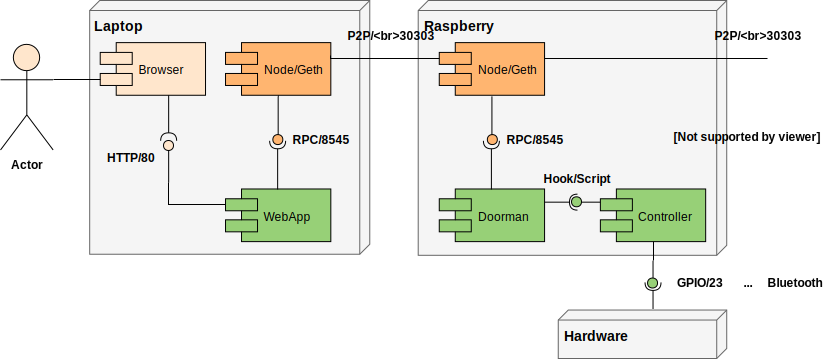
\includegraphics[width=.95\textwidth]{Aufbau_Komponenten_Interface}
\caption{Komponenten und Schnittstellen}
\label{fig:Komponenten und Schnittstellen}
\end{figure}

\section{Komponenten}
\label{sys_sec:Komponenten}
Folgend werden alle im Lokkit System vorhandenen Komponenten, deren Abhängigkeiten und vorgenommene Konfiguration erklärt.

\subsection{Geth}
\label{sys_subsec:Geth}
\begin{itemize}
    \item Konfiguration von Geth
    \item Funktionsweise blockchain KURZ
\end{itemize}

\subsection{Smart Contracts}
Die Datenhaltung und Businesslogik des Lokkit Systems liegt auf der Blockchain in Form von Smart Contracts.
\subsubsection{Rentable}
\label{sys_subsubsec:Rentable}
Eine Instanz dieses Contracts spiegelt ein mietbares Objekt wieder.

\paragraph{Attribute}
\label{sys_para:Rentable_Attribute}
Attribute eines Rentable können gelesen und gesetzt werden. Lesen wird durch die automatische Lesefunktion von Solidity gemacht, gesetzt werden die Attribute durch eine entsprechende Funktion, die den prefix \emph{set} hat und den neuen Wert als einzigen Parameter annimmt. Wichtig zu beachten ist, dass die Funktion zum Ändern des Owners nicht setOwner sondern \emph{transferOwnership} heisst. Dieser Name widerspiegelt die Tatsache, dass der Besitz transferiert wird und sollte nicht leichtfertig mit einer \emph{set} Funktion verwechselt werden. Wenn eine Eigenschaft mittels einer \emph{set} Funktion verändert wird, wird das OnUpdate\emph{X} Event ausgelöst, wobei X für die veränderte Eigenschaft steht. 

\begin{longtable}{@{}llL{9cm}@{}}
\caption{Rentable Eigenschaften}\label{tbl:Rentable_Eigenschaften}\\
\toprule
Name & Typ & Beschreibung \\ \midrule
owner & address   & Besitzer des Rentable Objektes. Kann Eigenschaften verändern und privilegierte Funktionen ausführen.\\
description & string   & Beschreibung des Rentable Objektes.\\
location & string   & Besitzer des Rentable Objektes. Kann Eigenschaften verändern und privilegierte Funktionen ausführen.\\
costPerSecond & uint   & Kosten des Rentables in Wei pro Sekunde.\\
deposit & uint   & Menge Wei, die hinterlegt werden muss. Wird zurückerstattet, wenn \emph{unclaim} oder \emph{forceUnclaim} aufgerufen werden (vgl. \ref{sys_para:claim_unclaim}).\\
\end{longtable}

\paragraph{Berechnung der Kosten}
Die totalen Kosten eines Rentable für einen Zeitraum werden durch zwei Faktoren bestimmt: die Kosten in wei pro Sekunde (vgl. \ref{sys_para:Rentable_Attribute}) und das zu hinterlegende Depot (vgl \ref{math:Rentable_Cost}). Sollte die überwiesene Menge Ether zu gross sein, wird der Überschuss in die \emph{pendingRefunds} (vgl. XX) der sendenden Adresse gutgeschrieben.

\begin{equation}
\label{math:Rentable_Cost}
totalCost = (rentDuration * costPerSecond) + deposit
\end{equation}

\paragraph{unclaim und forceUnclaim}
\label{sys_para:claim_unclaim}
Um die regelkonforme Rückgabe eines Rentables festzustellen, muss vom Mieter die Funktion \emph{unclaim} aufgerufen werden (vgl. \ref{tbl:Rentable_Funktionsuebersicht}). Damit bestätigt der Mieter, dass das Rentable nicht länger verwendet wird. Sollte der Mieter nicht unclaim aufrufen, kann der \emph{owner} zu einem Zeitpunkt nach der Reservation die Funktion \emph{forceUnclaim} aufrufen (vgl. \ref{tbl:Rentable_Funktionsuebersicht}), um das Depot seinen \emph{pendingRefunds} gutzuschreiben.

\paragraph{pendingRefunds}
Falls zu viel Ether an den Contract überwiesen wird oder eine Rückerstattung des \emph{deposit} erwirkt wurde, werden die Beträge in die \emph{pendungRefunds} des Rentables eingetragen. Diese können explizit aus deom Smart Contract abgehoben werden.\cite[Miscellaneous/Introduction to Smart Contracts]{solidity.readthedocs.io}

\paragraph{Funktionsübersicht}

L: Lesefunktion, S: Schreibfunktion, C: Konstruktor, E: Event

\begin{longtable}{@{}lcL{9cm}@{}}
\caption{Rentable Lesefunktionen}\label{tbl:Rentable_Funktionsuebersicht}\\
\toprule
Name & Typ & Beschreibung \\ \midrule
allReservations     & L   & Gibt alle Reservationen als Array zurück. Eine Reservation besteht aus einem Array mit drei Einträgen: Startzeit, Endzeit, Ob die aufrufende Adresse der Mieter ist.\\
 & & Parameter: keine \\\midrule
reservedAt          & L   & Gibt zurück, ob das Rentable am gegebenen Zeitpunkt \emph{time} reserviert ist.\\ & & Parameter: \emph{time} \\\midrule
reservedBetween     & L   & Gibt zurück, ob das Rentable zwischen den gegebenen Zeitpunkten \emph{start} und \emph{end} reserviert ist.\\ & & Parameter: \emph{start}, \emph{end} \\\midrule
currentRenter       & L   & Gibt die Adresse des momentanen Mieters zurück. Wenn das Rentable momentan nicht vermietet ist, wird 0 zurückgegeben.\\ & & Parameter: keine \\\midrule
costInWei           & L   & Gibt die Kosten in Wei für die Zeit zwischen \emph{start} und \emph{end} zurück.\\ & & Parameter: \emph{start}, \emph{end} \\\midrule
myPendingRefund     & L   & Gibt zurück, wie viel Ether die aufrufende Adresse noch zur Verfügung hat.\\ & & Parameter: keine \\ \midrule
currentReservation  & L   & Gibt die momentane Reservation zurück als Array mit drei Einträgen: Startzeit, Endzeit, Ob die aufrufende Adresse der Mieter ist.\\ & & Parameter: keine \\\midrule
transferOwnership   & S   & Setzt den \emph{owner} des Rentables auf die angegebene Adresse \emph{newOwner}.\\ & & Parameter: \emph{newOwner} \\\midrule
setDescription   & S   & Setzt \emph{description} des Rentables auf den angegebenen Text \emph{newDescription}.\\ & & Parameter: \emph{newDescription} \\\midrule
setLocation   & S   & Setzt die \emph{location} des Rentables auf den angegebenen Text \emph{newLocation}.\\ & & Parameter: \emph{newLocation} \\\midrule
setCostPerSecond   & S   & Setzt die \emph{costPerSecond} des Rentables auf die angegebene Menge \emph{newCostPerSecond}.\\ & & Parameter: \emph{newCostPerSecond} \\\midrule
setDeposit   & S   & Setzt das \emph{peposit} des Rentables auf die angegebene Menge \emph{newDeposit}.\\ & & Parameter: \emph{newDeposit} \\\midrule
rent                & S   & Mietet das Rentable zwischen \emph{start} und \emph{end} für die sendende Adresse.\\ & & Parameter: \emph{start}, \emph{end} \\\midrule
unclaim         & S   & Retourniert ein Rentable während die gemietete Zeit noch nicht abgelaufen ist. Der bezahlte Betrag für die zusätzliche Zeit wird gleichmässig zwischen \emph{renter} und \emph{owner} aufgeteilt. Das \emph{deposit} wird dem refund des \emph{renter}s gutgeschrieben.\\ & & Parameter: keine \\\midrule
forceUnclaim         & S   & Retourniert alle Reservations, die in der Vergangenheit liegen und auf welchen nicht unclaim aufgerufen wurde. Das \emph{deposit} wird dem refund des \emph{owner}s gutgeschrieben.\\ & & Parameter: keine \\\midrule
withdrawRefunds     & S   & Hebt alle bestehenden Rückerstattungen einer Adresse vom Rentable ab und überweist sie auf das Konto der sendenden Adresse\\ & & Parameter: keine \\\midrule
Rentable            & C   & Erstellt ein neues Rentable mit den angegebenen Parametern und der sendenden Adresse als \emph{owner}.\\ & & Parameter: \emph{pdescription}, \emph{plocation}, \emph{pcostPerSecond}, \emph{pdeposit} \\ \midrule
OnRent              & E   & Wird ausgelöst, wenn versucht wird, das Rentable zu mieten (vgl. Funktion \emph{rent}). \emph{success} gibt an, ob die Reservation erfolgreich war.\\ & & Parameter: \emph{success}, \emph{renter}, \emph{start}, \emph{end}, \emph{msg} \\ \midrule
OnUpdateOwner              & E   & Wird ausgelöst, wenn \emph{owner} durch die \emph{transferOwnership} Funktion verändert wird.\\ & & Parameter: \emph{oldOwner}, \emph{newOwner} \\ \midrule
OnUpdateDescription              & E   & Wird ausgelöst, wenn \emph{description} durch die \emph{setDescription} Funktion verändert wird.\\ & & Parameter: \emph{oldDescription}, \emph{newDescription} \\ \midrule
OnUpdateLocation              & E   & Wird ausgelöst, wenn \emph{location} durch die \emph{setLocation} Funktion verändert wird.\\ & & Parameter: \emph{oldLocation}, \emph{newLocation} \\ \midrule
OnUpdateCostPerSecond              & E   & Wird ausgelöst, wenn \emph{costPerSecond} durch die \emph{setCostPerSecond} Funktion verändert wird.\\ & & Parameter: \emph{oldCostPerSecond}, \emph{newCostPerSecond} \\ \midrule
OnUpdateDeposit              & E   & Wird ausgelöst, wenn \emph{deposit} durch die \emph{setDeposit} Funktion verändert wird.\\ & & Parameter: \emph{oldDeposit}, \emph{newDeposit} \\
\bottomrule
\end{longtable}


\subsection{Webapp}
\label{sys_subsec:Webapp}
Die Webapp für Lokkit stellt eine Gerätunabhängige Benutzeroberfläche für die Interaktion mit dem Lokkit System zur Verfügung. Es wird mindestens ein Account, mit genügend Ether, vorausgesetzt, um mit den Rentable Objekten interagieren zu können.

\paragraph{}
Das Webapp basiert auf \emph{NodeJS} und benutzt \emph{VueJS} mit Material Design für die Benutzeroberfläche. Um mit der Blockchain zu interagieren wird die \emph{Web3.js} Library verwendet. Die Abbildung \ref{fig:Aufbau der Webapp} zeigt eine grobe Übersicht über die verschiedenen Elemente.



\begin{figure}[H]
\centering
\includegraphics[width=.95\textwidth]{Aufbau_Webapp}
\caption{Aufbau der Webapp}
\label{fig:Aufbau der Webapp}
\end{figure}

\subsubsection{NodeJS}
\subsubsection{VueJS}
\subsubsection{Ethereum Node}
Die Vorbedingung zur Verwendung der Webapp ist eine laufende und korrekt konfigurierte Ethereum Node auf demselben Gerät, die die jsonrpc Schnittstellen \emph{eth}, \emph{shh}, \emph{personal} auf dem Port 8545 zur Verfügung stellt.

\subsection{Android App}
\label{sys_subsec:Android_App}
Die Android App startet und administriert eine Ethereum Node mit dem Lokkit Genesis Block, um die Verwendung vom Lokkit Webapp (vgl. \ref{sys_subsec:Webapp}) auf einem Androidgerät zu ermöglichen.

Wenn die Android App das erste mal gestartet wird, wird der Lokkit Service gebunden und die Activity nach einem Passwort für den Account gefragt (vgl. \ref{fig:android_sequence_start}). Bei nachfolgenden Starts wird der erstellte Account geladen und die Activity nach dessen Password gefragt. Wenn die Verbindung erfolgreich hergestellt werden konnte, wird das Webapp geladen.

\begin{figure}[H]
\centering\small
\setlength{\tabcolsep}{0mm}	% alle Spaltenränder auf 0mm
\begin{tabular}{c@{\hspace{12mm}}c} % mittlerer Abstand = 12mm
  \includegraphics[width=.48\textwidth]{android_sequence_start_new} &
  \includegraphics[width=.42\textwidth]{android_sequence_start_existing} \\
  (a) & (b)
\end{tabular}
%
\caption{erster Start (a), spätere Starts (b)}
\label{fig:android_sequence_start}
\end{figure}

\subsubsection{Statusgo}
Diese Subkomponente implementiert das Ethereum Protokoll und weitere Funktionalität von status-im. Die API kann über die statische Klasse \emph{Statusgo}\footnote{Im Paket com.github.status\_im.status\_go.cmd zu finden} in Java verwendet werden. Diese Library implementiert das gesamte Ethereum Protokoll und die light node.\cite[wiki/Build-Process-Explained]{github.com/status-im/status-go}

\subsubsection{Lokkit Service}
Der Lokkit Service konsumiert das statusgo-android Modul. Der Service wird bei Start der Applikation gestartet und bei Beenden der Applikation gestoppt. Der Service sendet und empfängt Intents (vgl. \ref{tbl:LokktService_SendIntents}, \ref{tbl:LokktService_ListenIntents}) für die Interaktion mit der Lokkit Activity (vgl. \ref{sys_subsubsec:Lokkit_Activity}).\cite[Bound Services]{developer.android.com}

Die Statusgo Library bedingt, dass eine erstellte Transaktion zuerst durch Statusgo freigegeben wird, bevor sie in die \emph{pending transactions} von geth aufgenommen wird (vgl. \ref{sys_subsec:Geth}). Dabei weist Statusgo jeder Transaktion eine id zu. Diese id ist spezifisch für Statusgo und hat keine Bedeutung im Ethereum Protokoll.

\begin{table}[H]
\centering
\caption{Intents, die vom Lokkit Service gesendet werden}
\label{tbl:LokktService_SendIntents}
\begin{tabular}{@{}L{3cm}L{2cm}L{10cm}@{}}
\toprule
action & extras & Beschreibung \\ \midrule
io.lokkit.\newline{}COMPLETE\newline{}\_TRANSACTION\newline{}\_FAILED & id, reason & Wird als Antwort auf io.lokkit.COMPLETE\_TRANSACTION gesendet, wenn eine Transaktion nicht bestätigt werden konnte. \\\midrule
io.lokkit.\newline{}COMPLETE\newline{}\_TRANSACTION\newline{}\_SUCCESSFUL & id & Wird als Antwort auf io.lokkit.COMPLETE\_TRANSACTION gesendet, wenn eine Transaktion erfolgreich bestätigt werden konnte. \\\midrule
io.lokkit.\newline{}LOGIN\newline{}\_SUCCESSFUL & - & Wird als Antwort auf io.lokkit.LOGIN gesendet, wenn das in io.lokkit.LOGIN gesendete Password für das Entsperren des gespeicherten Accounts verwendet werden konnte. \\\midrule
io.lokkit.\newline{}RECOVER\newline{}\_ACCOUNT & address, mnemonic & Wird gesendet, wenn der Service beim Start einen Account findet. Muss mit io.lokkit.LOGIN beantwortet werden. \\\midrule
io.lokkit.\newline{}REQUIRE\newline{}\_ACCOUNT & - & Wird gesendet, wenn ein Account gefunden wurde. Muss mit io.lokkit.LOGIN beantwortet werden. \\\midrule
io.lokkit.\newline{}COMPLETE\newline{}\_TRANSACTION & id & Da der Demonstrator nur die Lokkit webapp bedient, wurde der Einfachheit halber diese Funktionalität umgangen, indem der Service die Nachfrage nach de Account sich selbst beantwortet. \\
\bottomrule
\end{tabular}
\end{table}

\begin{table}[H]
\centering
\caption{Intents, die von Lokkit verarbeitet werden}
\label{tbl:LokktService_ListenIntents}
\begin{tabular}{@{}L{3cm}L{2cm}L{10cm}@{}}
\toprule
action & extras & Beschreibung\\ \midrule
io.lokkit.\newline{}COMPLETE\newline{}\_TRANSACTION & id, password & Bestätigt die Transaktion mit id id durch Verwendung des momentanen Accounts (vgl. Statusgo.Login()) und des angegebenen Passworts. Die Transaktion wird erst durch Senden dieses Intents in die Liste der pending transactions aufgenommen. Aufruf wird bestätigt durch einen Intent mit action io.lokkit.COMPLETE\_TRANSACTION\_SUCCESSFUL, falls erfolgreich oder io.lokkit.COMPLETE\_TRANSACTION\_FAILED falls nicht erfolgreich. \\\midrule
io.lokkit.\newline{}DISCARD\newline{}\_TRANSACTION  & id           & Verneint die Transaktion mit id id. Diese Funktionalität kann verhindern, dass ohne Erlaubnis des Benutzers eine Transaktion von einer DAPP ausgelöst wird. Aufruf wird nicht bestätigt.\\\midrule
io.lokkit.\newline{}LOGIN & password     & Meldet den persistierten Benutzer an. Aufruf wird bestätigt durch einen Intent mit action io.lokkit.LOGIN\_SUCCESSFUL, falls erfolgreich oder io.lokkit.RECOVER\_ACCOUNT falls nicht erfolgreich.
\\ \bottomrule
\end{tabular}
\end{table}

\subsubsection{Lokkit Activity}
\label{sys_subsubsec:Lokkit_Activity}
Wenn die Lokkit App gestartet wird, wird die Lokkit Activity geöffnet. Diese Activity dient dazu, die Interaktion des Benutzers mit dem Lokkit Service sicherzustellen. Falls der Lokkit Service Eingaben benötigt, wird die Activity benachrichtig und wird dementsprechend den Benutzer nach der Eingabe fragen, bspw. wenn ein Passwort für einen neuen Account angegeben werden muss (vgl. \ref{fig:sys_android_new_account}).

\begin{figure}[H]
\centering
\includegraphics[width=.40\textwidth]{android_new_account}
\caption{Beispielansicht: Activity fragt den Benutzer nach einem Passwort für einen neuen Account}
\label{fig:sys_android_new_account}
\end{figure}



\subsection{Doorman}
Doorman verbindet auf eine ethereum node, die die shh und eth Protokolle enabled hat und hört auf Whisper v5 Nachrichten für die in der Konfiguration definierten Rentables. Wenn die payload der Nachrichten der Definition in der Real-Time Kommunikationsschnitstelle (vgl. \ref{sys_subsec:Real_Time_Kommunikationsschnittstelle}) entsprechen, wird ein Script ausgeführt, das als Parameter die Adresse des Rentables, sowie das command (vgl. \ref{sys_subpara:Command}) erhält.

\subsubsection{Konfiguration}
\label{sys_subsec:Doorman_Konfiguration}
Die Konfiguration des Doorman wird aus einer yml Datei\footnote{https://fdik.org/yml/} gelesen. Die Datei besitzt einen root mit Namen \emph{doorman} und Attribute für die Ethereum Node, verwendete Rentable Smart Contract Adressen und auszuführendes Script bei Erhalt einer validen Nachricht.
\begin{lstlisting}[language=yml,caption={Beispielkonfiguration für Doorman}]
doorman:
    node_ip: 127.0.0.1
    node_rpc_port: 8545
    rentable_addresses:
        - "0xf16801293f34fc16470729f4ac91185595aa6e10"
        - "0x298345dddd494c51061da2ae137df3129ce14b69"
    script: open_close_device.bat
\end{lstlisting}

\paragraph{node\_ip}
Die Url der Ethereum Node, zu der eine Verbindung aufgebaut werden soll. Diese Node muss das shh Protokoll und auch die shh API aktiviert haben (vgl. \ref{para:Whisper}). Die Adresse ist als IP anzugeben. Informationen zum Protokoll wie \emph{http://} sind auszulassen.
\paragraph{node\_rpc\_port}
Der Port, auf dem Doorman zu der Ethereum Node verbinden soll. Der Standardport ist 8545.
\paragraph{rentable\_address}
Die Adressen der Smart Contracts vom typ Rentable (vgl. \ref{sys_subsubsec:Rentable}), auf deren Nachrichten gehört werden sollen. Wird eine ungültige Rentable Adresse angegeben, werden die Befehle nicht ausgeführt.
\paragraph{script}
Das script, das ausgeführt werden soll.

\subsection{Controllers}
\subsubsection{Nuki}
\subsubsection{Schloss Marke Eigenbau}

\section{Interne Schnittstellen}
In diesem Abschnitt werden die internen Schnittstellen des Lokkit Systems beschrieben.

\subsection{Real-Time Kommunikationsschnittstelle}
\label{sys_subsec:Real_Time_Kommunikationsschnittstelle}
Diese Schnittstelle dient der Echtzeitkommunikation zwischen dem Webapp (vgl. \ref{sys_subsec:Webapp}) und dem Doorman (vgl. \ref{sys_subsec:Doorman}). Sie bedient sich kryptografischer Funktionen aus der Web3 Library, um die Validität des Absenders zu validieren.

\subsubsection{Aufbau der Nachricht}
Für das gesamte von Whisper v5 versendete Packet wird der Ausdruck \emph{Envelope} verwendet. Die darin enthaltene textbasierte Nachricht, die einen validen JSON-String beinhaltet, wird als \emph{Payload} bezeichnet. Da Whisper v5 nur textbasierte Payloads unterstützt, wurde eine Nachricht im \acrshort{JSON} Format definiert, die eine strukturierte Möglichkeit zur Datenübermittlung ermöglicht. Diese wird übermittelt, indem sie vom Sender zu einer String-Repräsentation umgewandelt wird und nach Erhalt beim Empfänger wiederum zu einem JSON geparst wird. Das definierte Objekt besitzt zwei Attribute: \emph{digest} (vgl. \ref{sys_para:Digest}), nachfolgend Diges und \emph{message} (vgl. \ref{sys_para:Message}), nachfolgend Message Objekt.

\begin{lstlisting}[language=json,caption={Beispiel einer Lokkit JSON Nachricht, deren \emph{digest} vom account \emph{0x55047206d03afef0d79bb2d90710bf9f23737860} erstellt wurde.}]
{
  digest: "0x06351aa8220219b621d7c2c5340110d3be147b92ef8035469df996762e021f512f4f8  30dee0ed1d59998b4bafaa3abb589668d940bdce867f7e6d83315a454af1b",
  message: {
    command: "open",
    key: "435712b75b3546c06ed5e9ab19fbc309c5f2e0a57701e56e39f43f449b6e72c9",
    rentableAddress: "0xbac41871cf121f6c02d345af52c82c83759a2e3b"
  }
}
\end{lstlisting}

\paragraph{Message}
\label{sys_para:Message}
Das Message Objekt innerhalb der Payload enthält drei Attribute: \emph{command}, \emph{rentableAddress} und \emph{key}. Funktional relevant für den Empfänger sind dabei nur command und rentableAddress. Das key Attribut ist eine zusätzliche Sicherheit, um Replay-Angriffe mit demselben Packet zu verhindern, bei welchen dasselbe Paket von einem anderen Sender versendet wird.
\subparagraph{Command}
\label{sys_subpara:Command}
Dieses Feld teilt den Befehl mit, den das mietbare Objekt ausführen soll. Abhängig von der jeweiligen Implementation des IoT Geräts kann dieses Feld andere Werte beinhalten. Im Beispiel von Lokkit werden \emph{lock} und \emph{unlock} für Schliessfächer geschickt. Weitere Befehle sind denkbar, die ebenfalls den Doorman als Empfänger verwenden.
\subparagraph{Rentable Address}
Damit der Empfänger weiss, welches mietbare Objekt von dem Befehl angesteuert werden soll, wird die gesamte Adresse mitgegeben. Alternativ könnte dieses Feld weggelassen werden und über das Topic der Nachricht bestimmt werden.

\subparagraph{Key}
\label{sys_para:Key}
Dieses Feld beinhaltet den öffentlichen Schlüssel eines asymmetrischen Schlüsselpaars des Senders. Derselbe Schlüssel muss zum signieren des Envelopes verwendet werden\footnote{Diese Signatur ist optional bei Whisper, wird jedoch für Lokkit Envelopes vorgeschrieben}. Der öffentliche Schlüssel des für die Signatur verwendeten Schlüsselpaars wird ebenfalls im Envelope als Feld \emph{sig} mitgeschickt. Bei einer validen Nachricht sind also das Feld \emph{key} des Message Objektes und das Feld \emph{sig} des Envelopes identisch\footnote{Für weitere Informationen, vgl. \ref{para:Replay_Attack}}.

\paragraph{Digest}
\label{sys_para:Digest}
Um den Digest eines Message Objekts zu erzeugen wird die Funktion \emph{web3.eth.sign} verwendet. Dieser Funktion wird als einziger Parameter die Stringrepräsentation des Message Objektes übergegeben. Bei entsperrtem Account liefert die Funktion einen 65 Byte Hash, den Digest, zurück. Dabei ist zu beachten, dass derselbe Account entsperrt ist, der auch das Rentable gemietet hat, an das diese Nachricht gesendet werden soll. Um herauszufinden, welche Ethereum Adresse den Digest des Message Objektes erzeugt hat, wird die Funktion \emph{web3.personal.ecRecover} verwendet. Diese nimmt als Parameter die Stringrepräsentation des Message Objektes und als zweiten Parameter den Digest. Als Rückgabewert liefert diese dann die Adresse, die die Signatur erstellt hat.

Wichtig dabei ist, dass die über Whisper erhaltenen JSON Objekte jeweils die Attribute in alphabetisch sortierter Reihenfolge beinhalten und über die javascript Funktion JSON.stringify serialisiert werden, bevor sie den kryptographischen Funtionen übergeben werden. Grund dafür ist, dass besagte sign Funktion eine Zeichenkette als Arugment nimmt und nicht ein Objekt. Die Verwendung von JSON.stringify versichert, dass der Eingabewert stets gleich strukturiert ist.

\begin{lstlisting}[language=javascript,caption={beispiel generate digest und ecRecover}]
// Sender
var message = { 'command': command, 'rentableAddress': rentableAddress, 'key': publicKey };
var messageBytes = web3.fromAscii(JSON.stringify(message));
var digest = web3.eth.sign(adi, messageBytes);

// Empfänger
var payload = JSON.parse(web3.toAscii(envelope.payload));
var signer = web3.personal.ecRecover(web3.fromAscii(JSON.stringify(payload.message)), payload.digest);
\end{lstlisting}
Dabei wird der Empfänger als Resultat von \emph{ecRecover} die Adresse erhalten, die beim Sender entsperrt war, als \emph{web3.eth.sign} aufgerufen wurde.

\subsubsection{Verteilung}
\label{sys_subsubsec:Verteilung}
Als key attribut des Envelopes wird ein symmetrischer Schlüssel mit dem Passwort \emph{lokkit} erstellt. Als Topic werden die ersten 4 Bytes der sha3 Checksumme der Adresse des Mietbaren Objektes mitgeschickt. Basierend auf diesen beiden Eigenschaften kann der Doorman (vgl. \ref{subsec:Doorman}) die für die angeschlossenen Geräte relevanten Nachrichten filtern.

\begin{lstlisting}[language=javascript,caption={Beispiel einer Whisper v5 Nachricht}]
var msg = "hello world";
var key = web3.shh.gensymkey();
var topic = 0xFFFF;
shh.post({key:key, topic:topic, payload:web3.fromAscii(msg)});
\end{lstlisting}


\begin{lstlisting}[language=javascript,caption={Beispiel eines Whisper v5 Filters}]
var shhPw = "lokkit";
var key = shh.addSymmetricKeyFromPassword(shhPw);
var topic = web3.sha3(rentableAddress).substr(0, 10);
var filterId = web3.shh.subscribe({type: 'sym', topics: [topic], key: key});
web3.shh.getFilterUpdates(filterId).forEach(function(err, result) {
    // result ist der envelope.
    console.log(result.sig);
    console.log(result.payload);
}
\end{lstlisting}

\section{Demonstrator Aufbau}
\label{sys_sec:Demonstrator_Aufbau}

\subsection{Notöffnung}

\subsection{Elektronik}


\begin{figure}
\centering
\includegraphics[width=.95\textwidth]{schaltplan.png}
\caption{Schaltplan des Demonstrators}
\end{figure}



\chapter{Installation \& Deployment}
\label{cha:Installation_Deployment}

In den folgenden Abschnitten wird erklärt wie das System aufgesetzt wird. Jede Komponente wird aus den Sourcen gebildet und dann auf den Raspberries installiert. Dazu wird zuerst erklärt wie die Raspberries in Betrieb genommen werden.

\section{Voraussetzungen für das Deployment}
Die nachfolgende Anleitung wurde unter einem aktuellen GNU/Linux System erfolgreich getestet. Grundsätzlich sind andere Systeme wie Windows oder MAC jedoch nicht ausgeschlossen und können für das Deployment ebenfalls verwendet werden. Dies jedoch auf eigene Verantwortung.

Konfigurationsübersicht zu diesem Zeitpunkt

\begin{table}[H]
\centering
\caption{Systemvorausetzungen um das Deployment durchzuführen}
\label{my-label}
\begin{tabular}{@{}lll@{}}
\toprule
Komponente 
& Version               
& Beschreibung                           
\\ \midrule
GNU/Linux  
& Ubuntu 16.04 (Xenial) 
& Basis System für das Deployment        
\\ \midrule
nodejs     
& 7.10.0                
& Voraussetzung für Webapp               
\\ \midrule
npm        
& 4.2.0                 
& Voraussetzung für Webapp               
\\ \midrule
git        
&  2.7.4                
& Zum Auschecken der Sourcen               
\\ \midrule
truffle    
& 3.2.4                 
& Für das Deployment der Smart Contracts 
\\ \midrule
geth       
& 1.6.2                 
& Ethereum Node                          
\\ \midrule
doorman    
&                       
&                           
\\ \midrule
Webapp     
&                       
&                                        
\\ \bottomrule
\end{tabular}
\end{table}

\paragraph{Herunterladen der Resourcen}

Die Lokkit Sourcen können wie folgt heruntergeladen werden:

\begin{lstlisting}[language=bash]
$ git clone https://github.com/lokkit/lokkit --recursive
\end{lstlisting}

\section{Aufsetzten der Raspberry Pi's}
Für jedes der drei Raspberry Pi's wurde ein eigenes Image erstellt. Die Images basieren auf dem offiziellen \emph{Raspbian Jessie Lite} Image \footnote{\url{https://www.raspberrypi.org/downloads/raspbian/}}.

\paragraph{}
\begin{description}
    \item[Lokkit Image 1] Dieses Image enthält die Konfiguration für den WLAN Hotspot und einen DNS/DHCP Server. Die anderen Raspberries verbinden sich zu diesem.
    \item[Lokkit Image 2] Dieses Image ist so konfiguriert, dass es sich mit dem HotSpot des Master Images verbindet.
    \item[Lokkit Image 3] Dieses Image ist bis auf den Hostnamen identisch mit dem Lokkit Image 2
\end{description}

\paragraph{}
Alle drei Images können z.B. mit \emph{dd} unter GNU/Linux auf eine MicroSD geflashed werden. 

\begin{lstlisting}[language=bash,caption={Beispiel \emph{dd} unter GNU/Linux}]
$ dd if=rasp-master.img of=/dev/sdd
$ dd if=rasp-node1.img of=/dev/sdd
$ dd if=rasp-node2.img of=/dev/sdd
\end{lstlisting}

Danach können die Raspberries mit dem Image gestartet werden und nach spätestens 5 Minuten sollte ein Hotspot \emph{lokkit} ersichtlich sein. Die Zugangsdaten für das WLAN können der Tabelle \ref{tbl:wlan_zugang} entnommen werden.  

\begin{table}[]
\centering
\caption{WLAN Zugangsdaten}
\label{tbl:wlan_zugang}
\begin{tabular}{@{}ll@{}}
\toprule
SSID    & Passwort \\ \midrule 
lokkit  & trust-no-one \\ \bottomrule
\end{tabular}
\end{table}


Nach erfolgreichem Verbinden mit dem \emph{lokkit} Hotspot ist es nun möglich auf die Raspberries über \emph{SSH} zuzugreifen. Im untenstehenden Beispiel wird eine Verbindung zum Master-RaspberryPi hergestellt. 

\begin{lstlisting}[language=bash,caption{SSH Verbindung mit Master}]
$ ssh master.lokkit.io -l pi
# oder auch
$ ssh 192.168.0.1 -l pi
\end{lstlisting}

Die Benutzer und Passwörter der Raspberry Pi's sind der Tabelle \ref{tbl:raspberry_zugang} zu entnehmen.

\begin{table}[]
\centering
\caption{SSH Zugang}
\label{tbl:raspberry_zugang}
\begin{tabular}{@{}lll@{}}
\toprule
Host              & Benutzer   & Passwort \\ \midrule
master.lokkit.io  & pi         & TrNoOnJuLo \\ \midrule
node1.lokkit.io   & pi         & TrNoOnJuLo \\ \midrule
node2.lokkit.io   & pi         & TrNoOnJuLo \\ \bottomrule
\end{tabular}
\end{table}


\paragraph{Netzwerk} 
Der Hotspot verwendet das \emph{192.168.0.0/24} Netzwerk. Falls Probleme mit der DNS-Auflösung auftreten, kann das Master Raspberry Pi auch direkt mit der IP \emph{192.168.0.1} angesprochen werden.

\paragraph{}
Nachdem nun die Raspberry Pi's aufgesetzt und gestartet sind, können die Softwarekomponenten installiert werden. Die nächsten Kapitel zeigen, wie dies geht.








\section{Aufsetzen der Private Chain}
Die Private Chain besteht aus Ethereum Nodes (geth), welche so konfiguriert sind, dass sie ein eigenes neues Netzwerk erstellen und nicht ins eigentliche Ethereum Netzwerk (Homestead) verbinden. Der \emph{geth}\footnote{\url{https://geth.ethereum.org/}} Client hat ein breites Interface und kann über die Kommandozeile konfiguriert werden. Um die Installation und die Konfiguration der Lokkit Private Chain zu vereinfachen wurde ein Debian Paket kreiert, welches auf dem Raspberry-Pi installiert werden kann und, dass den \emph{geth} Client mit allen benötigten Parameter aufsetzt und initialisiert. Nachfolgend wird gezeigt, wie das Debian Paket erstellt und auf den Raspberry Pi's installiert wird. 

\subsection{Builden der Debian Pakete}
Zuerst muss ins Repository \emph{chain} gewechselt werden. Dann können die Pakete folgendermaßen gebuildet werden:

\begin{lstlisting}[language=bash]
$ cd chain # ins Verzeichnis wechseln
$ debuild -us -uc # erstellt 2 Pakete ../lokkit-chain*.deb
\end{lstlisting}

Das Paket \emph{lokkit-chain-no-mine} kann dann auf die Raspberry Pi's kopiert und installiert werden. Das nächste Code Snippet muss für jedes Raspberry Pi durchgeführt werden.

\begin{lstlisting}[language=bash]
$ scp ../lokkit-chain-no-mine*.deb pi@master.lokkit.io:

$ ssh pi@master.lokkit.io
pi@master:~ $ sudo su
Passwort: 
pi@master:~ $ dpkg -i lokkit-chain-no-mine*.deb
\end{lstlisting}

\paragraph{}
Somit ist die Private Chain auf den Raspberry Pi's installiert und lauffähig. Sie ist jedoch noch leer, sprich es gibt noch keinen Miner, der Blöcke mined. Analog zur Installation der Raspberry Pi's muss nun noch die Miner-Hardware installiert werden. Dazu wird das Paket \emph{lokkit-chain-mine} verwendet. Das Endresultat ist eine Private Chain bestehend aus fünf Nodes. Zwei Nodes auf der Miner-Hardware und jeweils ein Node pro Raspberry Pi.

\section{Smart Contracts installieren}
Um die drei Rentable Contracts auf der Blockchain zu veröffentlichen, muss in das Repository \emph{contracts} gewechselt werden. Anschliessend kann mittels \emph{truffle} die Contracts deployed werden. 

\paragraph{}
Damit \emph{truffle} die Contracts veröffentlichen kann, muss der erste Account auf dem Master-Rapsberry entsperrt werden. Zu diesem Zweck muss auf dem Raspberry Pi eingeloggt werden und mittels \emph{geth attach} der erste Account entsprerren. Das untenstehende Code Snippet illustriert das Vorgehen. 

\begin{lstlisting}[language=bash,label={lst:rentable_deployment},caption={Deployment der Contracts}]
$ ssh master.lokkit.io -l pi 
pi@master:~ $ geth attach
personal.unlockAccount(personal.listAccounts[0])
pi@master:~ $ exit
$ exit

# Nun können die Contracts mit truffle veröffentlicht werden
$ cd contracts # ins Verzeichnis wechseln
$ truffle deploy --network lokkit
Using network 'lokkit'.

Running migration: 1_initial_migration.js
  Replacing Migrations...
  Migrations: 0x9624922904e8907373b23dfbe7723be094abf5d6
Saving successful migration to network...
Saving artifacts...
Running migration: 2_deploy_contracts.js
  Replacing Rentable...
  Rentable: 0x58b5e51386b46d018dcd0a3db91a6c69fed20ea8
  Replacing Rentable...
  Rentable: 0xde93b2965af6a49161f597604c600af9ea07883a
  Replacing Rentable...
  Rentable: 0x75105e510adf9fa0b1b1a5d35f9d8594ad36d8ed
Saving successful migration to network...
\end{lstlisting}

\noindent 
Die Adressen der veröffentlichten Rentables sind im Konsolenoutput von \emph{truffle} ersichtlich (vgl. \ref{lst:rentable_deployment}). Diese Adressen können nun mittels QrCode Generator\footnote{Z.B.: \url{http://goqr.me/de/}} gespeichert und ausgedruckt werden. Der Demonstrator hat für jedes Schliessfach auf der Vorderseite Platz für einen solchen.

\section{Webapp}
Die Webapp wird ebenfalls per Debian Paket auf dem Master Raspberry Pi installiert. Nach erfolgreicher Installation ist sie unter \url{https://webapp.lokkit.io} aufrufbar. Um mit der Installation zu starten muss ins Repository \emph{webapp} gewechselt werden. Anschliessend kann das Debian Paket gebuildet und auf das Raspberry Pi kopiert und installiert werden. Der folgende Code illustriert das Vorgehen:

\begin{lstlisting}[language=bash]
$ cd webapp # ins Verzeichnis wechseln
$ debuild -us -uc # erstellt 1 Paket ../lokkit-webapp*.deb
$ scp ../lokkit-webapp*.deb pi@master.lokkit.io:
$ ssh pi@master.lokkit.io
pi@master:~ $ dpkg -i lokkit-webapp*.deb
\end{lstlisting}

Zum Testen kann jetzt per Web Browser auf \url{https://webapp.lokkit.io} zugegriffen werden.

\section{Doorman}
Doorman muss auf allen drei Raspberry Pi's installiert und dann unterschiedlich konfiguriert werden. Die Installation erfolgt ebenfalls durch ein Debian Paket.

\begin{lstlisting}[language=bash]
$ cd doorman # ins Verzeichnis wechseln
$ debuild -us -uc # erstellt 1 Paket ../lokkit-doorman*.deb
$ scp ../lokkit-doorman*.deb pi@master.lokkit.io:
$ ssh pi@master.lokkit.io
pi@master:~ $ dpkg -i lokkit-doorman*.deb
\end{lstlisting}

Nach erfolgreicher Installation von Doorman, muss dieser jeweils mit der, für das Schliessfach angepassten, Konfiguration gestartet werden. Die Konfiguration enthält jeweils die Adresse des entsprechenden Rentables und verweist auf ein Script, das das Schloss ansprechen kann. Beim Locker 2 und 3 sind die Schlösser identisch, und somit auch das Script. 

\paragraph{}
Die Konfiguration von Doorman liegt unter \emph{/etc/lokkit/doorman.yaml} und muss folgenden Inhalt haben:

\begin{lstlisting}[language=yaml,caption={Doorman-Konfiguration für Locker 2 und 3}]
doorman:
    node_ip: 127.0.0.1
    node_rpc_port: 8545
    rentable_addresses:
        - "0x58b5e51386b46d018dcd0a3db91a6c69fed20ea8" # Achtung: Korrekte Adresse eintragen
    symmetric_key_password: lokkit
    script: /opt/lokk.sh
\end{lstlisting} 

\paragraph{} 
Für Locker 1 und 2 muss noch die Datei \emph{/opt/lokk.sh} erstellt werden, welches den GPIO ansteuert und somit das Schloss öffnen kann.

\begin{lstlisting}[language=bash,caption={Script für Locker 2 und 3, das von Doorman aufgerufen wird}]
#!/bin/sh

port=17 # Verwendeter GPIO Port
echo Initializing port $port
echo $port > /sys/class/gpio/export
echo "out" > /sys/class/gpio/gpio${port}/direction
echo Initialization done

# Öffnen des Schlosses
echo "1" > /sys/class/gpio/gpio${port}/value

# Warten von 3 Sekunden
sleep 3

# Schliessen
echo "0" > /sys/class/gpio/gpio${port}/value
\end{lstlisting} 

\paragraph{}
Auf dem Locker 1 muss ein anderes Script hinterleget werden, welches das Nuki Schloss anprechen kann. Zuerst muss aber das Script auf dem Raspbery-Master (Locker 1) installiert werden. Dazu wird das Repository \emph{nuki} direkt auf das Master Raspberry kopiert. Anschliessend wird in der Doorman Konfiguration das Script auf /opt/nuki/lokk.sh geändert.

\begin{lstlisting}[language=bash]
$ scp nuki pi@master.lokkit.io:
$ ssh pi@master.lokkit.io
pi@master:~ $ sudo mv nuki /opt
\end{lstlisting}


\section{Android App}
Die Android App ist das letzte Stück dieser Kette. Sie kann unter \url{https://lokkit.io/download} heruntergeladen und installiert werden.
%\chapter{Projektmanagement}

\section{Dokumentinfos}
versionsupdate für Risikobeurteilung etc.

\section{Projektorganisation}
ziele, team (rollen, zuständigkeiten), 
\subsection{Projektziele}
Das Ziel dieses Projektes ist es, bestehende Blockchain Technologien zu recherchieren und zu analysieren und basierend auf dieser Vorarbeit einen Demonstrator zu konzipieren und zu implementieren, der die Blockchain Technologie mit IoT Geräten verbindet. Dieser entwickelte Demonstrator wird der Hochschule Luzern als Aktiva übergeben und soll als solcher weiterverwendet werden können. Die konkrete Aufgabenstellung für den Demonstrator wurde ebenfalls im Rahmen dieses Projektes vom Projektteam entwickelt.

\subsection{Rollen \& Zuständigkeiten}
\subsubsection{Projektteam}
Domi \& Andi

\subsubsection{Hochschule Luzern \& Experte}
Weingärtner, Hüsler, Experte

\section{Projektführung}
Im diesem Projekte wurden die vier klassischen Phasen aus SoDa\footnote{Software Development agile, hslu 2017} grundsätzlich befolgt, jedoch wird in diesem Projektmanagementplan eine andere Terminologie für die Phasen verwendet, um die explorative Methodologie dieses Projektes zu betonen.

\subsection{Projektplanung}
\#todo: plan inkl. meilensteine einfügen (aus mid term präsi, evtl updaten)

\paragraph{Initialisierung 24. März}
(Aufgabenstellung definiert) Bis am 24. März war die Recherche und Ausarbeitung einer konkreten Aufgabenstellung geplant, die anschliessend implementiert wird. Ein Grobkonzept (\#TODO: müssen wir hier ein ein dokument haben oder genügt ein Kapitel ''Grobkonzept'' im Bericht?) sollte vorliegen.

Diese Aufgabenstellung wurde am 13. März dem Auftraggeber mitgeteilt und am 14. März besprochen und angenommen (\#todo: siehe email vom 14.3)

\#todo: kommentare des Auftraggebers: siehe Notizen

\#todo: verweis auf requirements für prototyp

\paragraph{Zwischenpräsentation 26. April}
(Prototyp lauffähig) Während er Prototypphase sollte ein definierter Prototyp implementiert werden, der an der Zwischenpräsentation am 26. April vorgeführt werden kann. Dies diente zum einen der raschen Entwicklung einer demonstrierbaren Funktionalität an den Auftraggeber und zum anderen dem Sammeln von konkreten Erfahrungen für das Projektteam im Bereich der Blockchain Technologien. Diese Erfahrungen konnten in der darauf folgenden Phase gewinnbringend eingesetzt und zur Verbesserung der bestehenden Funktionalität verwendet werden.

Der Prototyp mit komplettem Systemdurchstich konnte demonstriert werden. Durch eine Webapp und lokal laufender Ethereum Node wurde demonstriert, dass die Kommunikation zwischen den Geräten funktioniert und auch die Echtzeitkommunikation mit dem Whisper v2 (\#todo: referenz zu whisper v5 update) Protokoll lauffähig ist.

\paragraph{Formelle Abgabe 9. Juni}
(Dokumentation abgabefertig \& Demonstrator lauffähig) Das Ende des Projektes war der 9. Juni 2017. An diesem Datum sollte der Demonstrator lauffähig, alle Funktionalität dokumentiert und die formellen Testfälle ausgeführt und entsprechend festgehalten sein. 

\#todo: Was hat alles funktioniert, was nicht?

\paragraph{Abschlusspräsentation 26. Juni}
Demonstrator "gehärtet" für Abschlusspräsentation und Demonstration (Verbesserungen bei Benutzerfreundlichkeit, Stabilität o.Ä.)
Funktional ist der Demonstrator und jegliche Dokumentation dessen abgeschlossen. Arbeiten, die am Demonstrator nach der Abgabe der Dokumentation gemacht wurden, beschränken sich nur auf den vorführbaren Wert für die Abschlusspräsentation und die Demonstration am 7. Juli.

\#todo: Hier werden wir allfällige weitere Änderungen referenzieren und als v1.1 an der Abschlusspräsi abgeben. Auch Geänderte Dokumente werden als v1.1 abgegeben.

\subsubsection{Recherchephase \emph{Initialisierungsphase}}
Im Rahmen des Kick-Off Meetings am 24. Februar übergab der Auftraggeber dem Projektteam den Projektauftrag für einen Demonstrator. Daraufhin wurde ein Rahmenplan erstellt und Meilensteine definiert. In der Recherchephase sollten bestehende Blockchain und IoT Technologien analysiert werden und darauf basierend ein Konzept für einen Demonstrator mit dem Auftraggeber besprochen und definiert werden.

\subsubsection{Prototypphase \emph{Konzeptionsphase}}
Das Ziel dieser Phase war es, einen Prototyp zu erstellen, der aufzeigt, dass die Aufgabenstellung so umgesetzt werden kann, wie sie im Konzept definiert wurde. Dabei ist zu beachten, dass das Blockchain Thema im Vordergrund stand. Bei der Umsetzung des Prototyps wurde nach dem explorativen Prinzip gearbeitet, wobei in Intervallen von einer Woche im Projektteam die momentane Situation analysiert und weitere Schritte festgelegt wurden. Hierbei griff das Projektteam sich verändernde Abhängigkeiten (siehe geth 1.6.1\^, status-im, web3 (whisper 5)) auf und versuchte ein limitiertes Set an Anforderungen für den Prototypen zu implementieren, um für die Realisierungsphase eine adäquate zusätzliche Menge Anforderungen definieren zu können.

Am Ende dieser Phase fand die Midterm Präsentation statt, bei der dem Auftraggeber die bisherigen Erfolge, namentlich der Prototyp, vorgeführt wurde. Diese Präsentation diente auch der Besprechung weiterer Anforderungen für die Realisierungsphase, in der der Demonstrator, inklusive der IoT Aspekte, vollumfänglich implementiert werden soll.

\subsubsection{Realisierungsphase}
Durch die Vorarbeit in den Recherche- und Prototyp- Phasen konnte für die Realisierungsphase eine Menge von Anforderungen definiert werden, die es zu implementieren gilt. Die Vorgehensweise in dieser Phase lehnt sich an das iterativ-inkrementelle Modell von SoDa an, verzichtet jedoch auf explizite Sprints und pflegt keine unterschiedlichen Product- und Sprintbacklogs. Wie auch in der Prototypphase wurden wöchentlich die Arbeiten besprochen und ad-hoc neue Prioritäten für die nächste Woche, basierend auf den noch offenen Anforderungen, definiert. Dies war möglich, da alle Anforderungen bereits in der Recherchephase definiert wurden. Technisch detaillierte User Stories zu definieren war nicht angebracht, da das know-how zur genügenden Fomrulierung solcher grösstenteils während der Realisierung erarbeitet werden musste. Auch die Grösse des Teams und die limitierte Zeitspanne rechtfertigt diese abgespeckte Interpretation von SoDa.

\subsubsection{Projektabschluss}
In der Projektabschlussphase wurden letzte Integrationstests ausgeführt, um die volle Funktionsfähigkeit des Demonstrators sicherzustellen und allfällige Abweichungen von der Konzeption zu dokumentieren. Weiter wurden die formalen Dokumente vervollständigt und abgeschlossen.

\subsection{Projektkontrolle}
Der Fortschritt wurde per eMail und in der Midterm Präsentation vom Projektteam an den Auftraggeber kommuniziert.

IST vs SOLL zustand und Massnahmen. (fakultativ)
bspw. bei Rückstand im Projektplan o.Ä.


\subsection{Verantwortlichkeiten}
Dominik Hirzel
\begin{itemize}
    \item Blockchain
    \item Smart Contracts
    \item Android App
    \item Dokumentation
\end{itemize}

\\Andreas Schmid
\begin{itemize}
    \item IoT
    \item Webapp
    \item Doorman
\end{itemize}


\section{Risikomanagement}
Das Risikomanagement wurde basierend auf der gängigen, und auch in SoDa definierten, Matrixmethode. Die horizontale Achse der Matrix entspricht der Auftretenswahrscheinlichkeit des Risikos, die vertikale Achse spiegelt die Schwere der Auswirkung wieder. Eine höhere Zahl bedeutet hierbei häufiger und schlimmer. Befindet sich die Wahrscheinlichkeit oder die Auswirkung eines Risikos im roten Bereich (vgl. \ref{tbl:Risikomatrix_Leer}), muss mindestens eine Mitigationsmassnahe getroffen werden, um die entsprechende Eigenschaft in den gelben Bereich zu verschieben. Bestenfalls würden Risiken durch besagte Massnahmen eliminiert werden.

\begin{table}[]
\centering
\caption{Risikomatrix Leer}
\label{tbl:Risikomatrix_Leer}
\begin{tabular}{@{}ccccccc@{}}
                             & 5 & \cellcolor[HTML]{DF8181} & \cellcolor[HTML]{DF8181} & \cellcolor[HTML]{DF8181} & \cellcolor[HTML]{DF8181} & \cellcolor[HTML]{DF8181} \\
                             & 4 & \cellcolor[HTML]{FFFA8F} & \cellcolor[HTML]{FFFA8F} & \cellcolor[HTML]{FFFA8F} & \cellcolor[HTML]{DF8181} & \cellcolor[HTML]{DF8181} \\
                             & 3 & \cellcolor[HTML]{92D050} & \cellcolor[HTML]{FFFA8F} & \cellcolor[HTML]{FFFA8F} & \cellcolor[HTML]{FFFA8F} & \cellcolor[HTML]{DF8181} \\
                             & 2 & \cellcolor[HTML]{92D050} & \cellcolor[HTML]{92D050} & \cellcolor[HTML]{FFFA8F} & \cellcolor[HTML]{FFFA8F} & \cellcolor[HTML]{DF8181} \\
\multirow{-5}{*}{\rotatebox[origin=c]{90}{Auswirkung}} & 1 & \cellcolor[HTML]{92D050} & \cellcolor[HTML]{92D050} & \cellcolor[HTML]{92D050} & \cellcolor[HTML]{FFFA8F} & \cellcolor[HTML]{DF8181} \\
                             &   & 1                        & 2                        & 3                        & 4                        & 5                        \\
                             &   & \multicolumn{5}{c}{Wahrscheinlichkeit}                                                                                              
\end{tabular}
\end{table}

\subsection{Übersicht}
Risiken werden für jede Phase als Übersicht vollumfänglich tabellarisch festgehalten. D.h., dass nicht nur neue Risiken erfasst sondern auch bestehende Risiken neu evaluiert (oder gestrichen) werden. Hierbei wird bewusst gewisse Redundanz zu Gunsten der Vollständigkeit auf einen Blick in Kauf genommen. Die Risiken werden mit einer Nummer versehen und ein Name zur einfacheren Identifikation definiert. Eine ausführliche Beschreibung der Risiken, eine Begründung für die Kategorisierung und allfällige Mitigationsmassnahmen werden anschliessend pro Risiko gelistet. Die Risiken werden in der Matrix vor und nach der Mitigationsmassnhamen dargestellt. Dabei ist die ausgegraute Nummer die Kategorisierung des Risikos vor und die voll schwarze Nummer dieselbe nach den Mitigationsmassnahmen. \#todo: wie schreibt man diesen satz besser? :/

\subsection{Risiken Recherchephase}
Während der Recherchephase waren die hauptsächlichen Risiken, dass die laufende Entwicklung an geth die zu implementierende Funktionalität für den Demonstrator einschränken kann.

\begin{table}[]
\centering
\begin{tabular}{lllll}
Nr & Risiko                                                  & A & W & Status \\
1  & geth unterstützt nicht alle Funktionalität              & 4          & 3                  & Neu    \\
2  & geth hat releaseverhindernde Fehler/Kompatibilität      & 5          & 2                  & Neu    \\
3  & Höhere Belastung des Projektteams durch Berufstätigkeit & 2          & 2                  & Neu    \\
4  & Temporärer Ausfall von github                           & 1          & 1                  & Neu    \\
5  & Temporärer Ausfall von sharelatex                       & 3          & 1                  & Neu   
\end{tabular}
\end{table}

\begin{table}[]
\centering
\caption{Risikomatrix Leer}
\label{tbl:Risikomatrix_Recherche}
\begin{tabular}{@{}ccccccc@{}}
                             & 5 & \cellcolor[HTML]{DF8181} & \cellcolor[HTML]{DF8181} & \cellcolor[HTML]{DF8181} & \cellcolor[HTML]{DF8181} & \cellcolor[HTML]{DF8181} \\
                             & 4 & \cellcolor[HTML]{FFFA8F} & \cellcolor[HTML]{FFFA8F} & \cellcolor[HTML]{FFFA8F} & \cellcolor[HTML]{DF8181} & \cellcolor[HTML]{DF8181} \\
                             & 3 & \cellcolor[HTML]{92D050} & \cellcolor[HTML]{FFFA8F} & \cellcolor[HTML]{FFFA8F} & \cellcolor[HTML]{FFFA8F} & \cellcolor[HTML]{DF8181} \\
                             & 2 & \cellcolor[HTML]{92D050} & \cellcolor[HTML]{92D050} & \cellcolor[HTML]{FFFA8F} & \cellcolor[HTML]{FFFA8F} & \cellcolor[HTML]{DF8181} \\
\multirow{-5}{*}{\rotatebox[origin=c]{90}{Auswirkung}} & 1 & \cellcolor[HTML]{92D050} & \cellcolor[HTML]{92D050} & \cellcolor[HTML]{92D050} & \cellcolor[HTML]{FFFA8F} & \cellcolor[HTML]{DF8181} \\
                             &   & 1                        & 2                        & 3                        & 4                        & 5                        \\
                             &   & \multicolumn{5}{c}{Wahrscheinlichkeit}                                                                                              
\end{tabular}
\end{table}

\paragraph{1}
\#todo: ??? mit 2 mergen?

\paragraph{2}
Sollte angedachte Funktionalität noch nicht in geth implementiert sein...

\paragraph{3}
Da alle Beteiligten des Projektteams neben diesem Projekt auch einer regulären Berufstätigkeit nachgehen, bei der sie eine zentrale Rolle in Entwicklungsteams einnehmen. Durch diese Beschäftigung ist es denkbar, dass der Arbeitgeber während der Projektzeit zusätzliche Anwesenheit verlangt.
\subparagraph{Mitigation}
Alle Beteiligten des Projektteams führen eine transparente Beziehung zu ihrem Arbeitgeber bezüglich ihrem Studium. Die Arbeitgeber unterstützen die Beteiligten des Projektteams in ihrem Studium. \#todo: umschreiben. Durch frühzeitige Kommunikation mit dem Arbeitgeber bezüglich fixen Terminen oder Projektabschlussphase (Intensivwoche) wird diesem Risiko entgegengewirkt. Auch Durch Belegung von wenigen weiteren Fächern wird die Belastung ausserhalb dieses Projektes gering gehalten.

\paragraph{5}


\subsection{Risiken Prototypphase}
Prototypphase...

\begin{table}[]
\centering
\caption{Risiken Recherchephase}
\label{}
\begin{tabular}{lllll}
Nr & Risiko                                                  & A & W & Status \\
1  & geth unterstützt nicht alle Funktionalität              & 4          & 3                  & Neu    \\
2  & geth hat releaseverhindernde Fehler/Kompatibilität      & 5          & 2                  & Neu    \\
3  & Höhere Belastung des Projektteams durch Berufstätigkeit & 2          & 2                  & Neu    \\
4  & Temporärer Ausfall von github                           & 1          & 1                  & Neu    \\
5  & Temporärer Ausfall von sharelatex                       & 3          & 1                  & Neu   
\end{tabular}
\end{table}

\begin{table}[]
\centering
\caption{Risikomatrix Leer}
\label{tbl:Risikomatrix_Recherche}
\begin{tabular}{@{}ccccccc@{}}
                             & 5 & \cellcolor[HTML]{DF8181} & \cellcolor[HTML]{DF8181} & \cellcolor[HTML]{DF8181} & \cellcolor[HTML]{DF8181} & \cellcolor[HTML]{DF8181} \\
                             & 4 & \cellcolor[HTML]{FFFA8F} & \cellcolor[HTML]{FFFA8F} & \cellcolor[HTML]{FFFA8F} & \cellcolor[HTML]{DF8181} & \cellcolor[HTML]{DF8181} \\
                             & 3 & \cellcolor[HTML]{92D050} & \cellcolor[HTML]{FFFA8F} & \cellcolor[HTML]{FFFA8F} & \cellcolor[HTML]{FFFA8F} & \cellcolor[HTML]{DF8181} \\
                             & 2 & \cellcolor[HTML]{92D050} & \cellcolor[HTML]{92D050} & \cellcolor[HTML]{FFFA8F} & \cellcolor[HTML]{FFFA8F} & \cellcolor[HTML]{DF8181} \\
\multirow{-5}{*}{\rotatebox[origin=c]{90}{Auswirkung}} & 1 & \cellcolor[HTML]{92D050} & \cellcolor[HTML]{92D050} & \cellcolor[HTML]{92D050} & \cellcolor[HTML]{FFFA8F} & \cellcolor[HTML]{DF8181} \\
                             &   & 1                        & 2                        & 3                        & 4                        & 5                        \\
                             &   & \multicolumn{5}{c}{Wahrscheinlichkeit}                                                                                              
\end{tabular}
\end{table}

\subsection{Risiken Realisierungsphase}
\subsection{Risiken Projektabschlussphase}


\section{Projektunterstützung}
\subsection{Tools}

\subsection{Konfigurationsmanagement}
Zusammenspiel der Versionen der Komponenten. --> Da nur eine Version veröffentlich wird, ist dies warscheinlich alles V1.0.0.


\section{Testkonzept}

%\chapter{Testing}

Dieses Dokument beschreibt wie sichergestellt wird, dass das System sich so verhaltet, wie es spezifiziert wird.

\subsection{Teststrategie}
Das System hat einen hoch komplexen Aufgbau und viele einzelne Komponenten. Umso wichtiger und komplizierter ist auch das Testing. Das Projekt wird auf drei Ebenen getestet. 

\vspace{.3cm}
\begin{description}
    \item[Unittests] Diese Tests sind vorallem während der Entwicklung einer Komponente wichtig.
    \item[Integrationstests] Eingige Komponenten sind stark von der Blockchain abhängig und müssen daher mit einer Blockchain-Instance getestet werden. Um dies zu vereinfachen wurde ein Dockerimage für eine lokale Blockchain erstellt  
    \item [Systemtests] Diese Tests testen das ganze System, inklusive aller Komponenten und der Blockchain. Mittels diesen Tests werden alle Use Cases validiert. Diese Tests gelten auch als Abnahmetests.
\end{description}

In den nachfolgenden Kapiteln werden die einzlnen Unittests, Integrationstests und Systemtests aufgelistet.

\subsection{Unittest}

\subsubsection{Smart Contract}
Die Tests können mit dem Befehl \emph{truffle test} auseführt werden.

\begin{table}[H]
\centering
\caption{Unittests des Smart Contracts Rentable}
\label{my-label}
\begin{tabular}{@{}L{.5cm}L{6cm}L{6cm}@{}}
\toprule
Nr. & 
Testname & 
Beschreibung 
\\ \midrule
1
& costPerSecond contract should be 7 
& Testet das Setzen von costPerSecond und dessen Berechnung 
\\ \midrule
2   
& descritption of contract should be 'leDescription'         
& Testet das \emph{Description}-Feld
\\ \midrule
3   
& location of contract should be 'leLocation'         
& Testet das \emph{Location}-Feld 
\\ \midrule
4   
& deposit of contract should be 500"         
& Testet das \emph{deposit}-Feld 
\\ \midrule
5   
& reserve (rent) the rentable         
& Testet die die \emph{reservedBetween} Funktion 
\\ \midrule
6   
& rent and check if reserved between         
& Testet die die \emph{rent} Funktion 
\\ \bottomrule
\end{tabular}
\end{table}

\begin{table}[H]
\centering
\caption{Unittests des Smart Contracts RentableDiscovery}
\label{my-label}
\begin{tabular}{@{}L{.5cm}L{6cm}L{6cm}@{}}
\toprule
Nr. & 
Testname & 
Beschreibung 
\\ \midrule
1
& can create contract using factory method
& Testet das Erzeugen von neuen \emph{Rentables} mittels Discovery Contract
\\ \bottomrule
\end{tabular}
\end{table}
\subsection{Integrationstests}
Die Integrationstests testen die einzelnen Komponenten gegen die Blockchain. 

\subsubsection{Doorman}

\paragraph{Voraussetzungen}

Um die Integrationstests von Doorman auszuführen muss folgendes Setup durchgeführt werden:

\begin{itemize}
    \item Auschecken der Doorman Resourcen
    \item Installieren der Abhängigkeiten
    \item Starten des Ethereum Nodes mittels Docker
    \item Veröffentlichen des Smart Contracts via truffle 
\end{itemize}

Danach können die Testfälle durchgespielt werden.
    
\begin{table}[H]
\centering
\caption{Test \#1: Starten von Doorman}
\label{my-label}
\begin{tabular}{@{}L{1.6cm}L{11cm}@{}}
\toprule
\textbf{Test \#1}
& Starten von Doorman mit Referenz zum veröffentlichten Contract
\\ \midrule
\textbf{Ablauf}
& 
\begin{enumerate}
    \item Eintragen der Addresse des veröffentlichten Contracts im Config file von Doorman
    \item Starten des Doormans
\end{enumerate}
\\ \midrule
\textbf{Ergebnis}
& Doorman startet und gibt folgendes Resultat auf der Konsole aus:
\begin{verbatim}
    Hoi ich bis der Dominik
\end{verbatim}
\\ \bottomrule
\end{tabular}
\end{table}

\begin{table}[H]
\centering
\caption{Test \#2: Doorman emfpängt Lock/Unlock-Befehl vom aktuellen Mieter}
\label{my-label}
\begin{tabular}{@{}L{1.6cm}L{11cm}@{}}
\toprule
\textbf{Test \#2}
& Doorman emfpängt Lock/Unlock-Befehl vom aktuellen Mieter
\\ \midrule
\textbf{Ablauf}
& 
\begin{enumerate}
    \item Mittels Truffle das Rentable für 5 min mieten
    \item Danach den Lock-Befehl ausführen
    \item Danach den Unlock-Befehl ausführen
\end{enumerate}
\\ \midrule
\textbf{Ergebnis}
& Doorman startet und gibt folgedes Resultat auf der Konsole aus:
\begin{verbatim}
    Hoi ich bis der Dominik
\end{verbatim}
\\ \bottomrule
\end{tabular}
\end{table}

\begin{table}[H]
\centering
\caption{Test \#3: Doorman emfpängt Lock/Unlock-Befehl von unbekanntem Account}
\label{my-label}
\begin{tabular}{@{}L{1.6cm}L{11cm}@{}}
\toprule
\textbf{Test \#3}
& Doorman emfpängt Lock/Unlock-Befehl von unbekanntem Account
\\ \midrule
\textbf{Ablauf}
& 
\begin{enumerate}
    \item Neuen Account auf der Node erstellen
    \item Lock Befehl signiert mit dem neuen Account absenden
    \item Unlock Befehl signiert mit dem neuen Account absenden
\end{enumerate}
\\ \midrule
\textbf{Ergebnis}
& Doorman startet und gibt folgedes Resultat auf der Konsole aus:
\begin{verbatim}
    Hoi ich bis der Dominik
\end{verbatim}
\\ \bottomrule
\end{tabular}
\end{table}

\subsubsection{Webapp}

\paragraph{Voraussetzungen}

Um die Integrationstests von der Webapp auszuführen muss folgendes Setup durchgeführt werden:

\begin{itemize}
    \item Auschecken der Webapp Resourcen
    \item Installieren der Abhängigkeiten
    \item Starten des Ethereum Nodes mittels Docker
    \item Starten der Webapp
    \item Veröffentlichen des Smart Contracts via truffle 
\end{itemize}

Danach können die Testfälle durchgespielt werden.


\begin{table}[H]
\centering
\caption{Test \#1: Hinzufügen eines Rentables }
\label{my-label}
\begin{tabular}{@{}L{1.6cm}L{11cm}@{}}
\toprule
\textbf{Test \#1}
& Hinzufügen eines Rentables
\\ \midrule
\textbf{Ablauf}
& 
\begin{enumerate}
    \item Füge das Rentable hinzu
    \item Schliesse den Browser und starte erneut
    \item Überprüfe, ob das Rentable noch hinzugefügt ist
\end{enumerate}
\\ \midrule
\textbf{Ergebnis}
& Das Rentable ist immer noch hinzugefügt.
\\ \bottomrule
\end{tabular}
\end{table}


\begin{table}[H]
\centering
\caption{Test \#2: Reservieren eines Rentables }
\label{my-label}
\begin{tabular}{@{}L{1.6cm}L{11cm}@{}}
\toprule
\textbf{Test \#2}
& Reservieren eines Rentables
\\ \midrule
\textbf{Ablauf}
& 
\begin{enumerate}
    \item Reserviere ein Rentable für 2 Minuten
    \item Überprüfe, ob die Reservations erfolgreich erscheint.
    \item Überprüfe, ob nach eintreten der Reservationszeit die Buttons Lock, Unlock erscheinen.
    \item Überprüfe, ob nach Aublauf der Reservation, die Buttons wieder verschwinden
\end{enumerate}
\\ \midrule
\textbf{Ergebnis}
& Die Reservation läuft erfolgreich durch. Beim Anbruch der Reservationsdauer sind Unlock und Lock ersichtlich. Nach Ablauf von ca 2. Minuten verschwinden die Buttons wieder. 
\\ \bottomrule
\end{tabular}
\end{table}


\begin{table}[H]
\centering
\caption{Test \#3: Fehleranzeige bei falscher Reservation}
\label{my-label}
\begin{tabular}{@{}L{1.6cm}L{11cm}@{}}
\toprule
\textbf{Test \#3}
& Fehleranzeige bei falscher Reservation
\\ \midrule
\textbf{Ablauf}
& 
\begin{enumerate}
    \item Reserviere ein Rentable in der Vergangenheit
    \item Überprüfe, ob eine entsprechende Fehlermeldung erscheint
\end{enumerate}
\\ \midrule
\textbf{Ergebnis}
& Das Rentable kann nicht reserviert werden, da eine Reservation in der Vergangenheit nicht möglich ist. 
\\ \bottomrule
\end{tabular}
\end{table}

\begin{table}[H]
\centering
\caption{Test \#4: Fehleranzeige bei Reservation mit Account ohne Ether}
\label{my-label}
\begin{tabular}{@{}L{1.6cm}L{11cm}@{}}
\toprule
\textbf{Test \#4}
& Fehleranzeige bei falscher Reservation
\\ \midrule
\textbf{Ablauf}
& 
\begin{enumerate}
    \item Wechsle den Account zu einem Account der 0 Ether besitzt.
    \item Reserviere ein Rentable in der Zukunft.
    \item Überprüfe, ob eine entsprechende Fehlermeldung erscheint
\end{enumerate}
\\ \midrule
\textbf{Ergebnis}
& Das Rentable kann nicht reserviert werden, da der Account nicht genügend Ether hat.
\\ \bottomrule
\end{tabular}
\end{table}
\subsection{Systemtests}
Die Systemtests testen das Gesamtsystem ausgehend vom Benutzer. Mit diesen Tests ist sichergestellt, dass der Demonstrator funktioniert.

\subsubsection{Voraussetzungen}
Für die folgenden Systemtests wird vorausgesetzt, dass das komplette System installiert und konfiguriert ist. Der Benutzer (Tester) besitzt ein Android Mobile Telefon und kann Applikationen aus dem Internet installieren.

Das Mobile Telefon muss mit dem Demonstrator WLAN verbunden sein.
Für jeden erstellten Account wird Ether vorausgesetzt.


\begin{table}[H]
\centering
\caption{Test \#1: Installieren des Mobile Apps}
\label{my-label}
\begin{tabular}{@{}L{1.6cm}L{11cm}@{}}
\toprule
\textbf{Test \#1}
& Installieren des Mobile Apps
\\ \midrule
\textbf{Ablauf}
& 
\begin{enumerate}
    \item Die Android-App via https://lokkit.io/download installieren
    \item Die Android-App starten (Benutzer muss erstellt werden)
    \item Einloggen des erstellten Benutzers
\end{enumerate}
\\ \midrule
\textbf{Ergebnis}
& Die Android-App ist erfolgreich auf dem Mobile Telefon installiert und kann gestartet werden. Der erstellte Benutzer kann eingeloggt werden.
\\ \bottomrule
\end{tabular}
\end{table}


\begin{table}[H]
\centering
\caption{Test \#2: Reservieren eines Rentables}
\label{my-label}
\begin{tabular}{@{}L{1.6cm}L{11cm}@{}}
\toprule
\textbf{Test \#2}
& Reservieren eines Rentables
\\ \midrule
\textbf{Ablauf}
& 
\begin{enumerate}
    \item Das Rentable über den QR-Code einscannen
    \item Das Rentable reservieren
    \item Ausführen von Lock und Unlock während der Reservationszeit
    \item Rückgabe des Rentables innerhalb der Reservationszeit
\end{enumerate}
\\ \midrule
\textbf{Ergebnis}
& Das Rentable konnte erfolgreich hinzugefügt werden. Die Reservation lief erfolgreich durch. Unlock und Lock haben entsprechend die Türe ge- und entsperrt. Das Rentable konnte erfolgreich zurückgeschoben werden.
\\ \bottomrule
\end{tabular}
\end{table}

\subsection{Testdruchführung am 04.06.2017}

\begin{table}[H]
\centering
\caption{Unittests des Smart Contracts Rentable}
\label{my-label}
\begin{tabular}{@{}L{4.5cm}L{4cm}L{4cm}@{}}
\toprule
Tests &
Tests erfolgreich & 
Tests fehlgeschlagen 
\\ \midrule
7 Unittests 
& 7
& 0
\\ \midrule
3 Integrationstests  
& 
& 
\\ \midrule
2 Systemtests
& 2
& 0
\\ \bottomrule
\end{tabular}
\end{table}

TODO: add all tests

%%%----------------------------------------------------------
\MakeBibliography
%%%----------------------------------------------------------

%%%Messbox zur Druckkontrolle
%\include{messbox}

\end{document}
